\documentclass[12pt,UTF8]{ctexart}
\usepackage{ctex,amsmath,amssymb,geometry,fancyhdr,bm,amsfonts,mathtools,extarrows,graphicx,url,enumerate,color,float,multicol,wasysym}
\usepackage{subfigure}
 
\allowdisplaybreaks[4]
% 加入中文支持
\newcommand\Set[2]{\left\{#1\ \middle\vert\ #2 \right\}}
\newcommand\Lim[0]{\lim\limits_{n\rightarrow\infty}}
\newcommand\LIM[2]{\lim\limits_{#1\rightarrow#2}}
\newcommand\Ser[1]{\sum_{n=#1}^\infty}
\newcommand{\SER}[2]{\sum_{#1=#2}^\infty}
\newcommand{\Int}[4]{\varint\nolimits_{#1}^{#2}#3\mathrm d#4}
\newcommand{\aIInt}[1]{\iint\limits_{#1}}
\newcommand{\IInt}[3]{\iint\limits_{#1}#2\mathrm d#3}
\newcommand{\varIInt}[4]{\iint\limits_{#1}#2\mathrm d#3\mathrm d#4}
\newcommand{\IIInt}[3]{\iiint\limits_{#1}#2\mathrm d#3}
\newcommand{\varIIInt}[5]{\iiint\limits_{#1}#2\mathrm d#3\mathrm d#4\mathrm d#5}
\newcommand{\LInt}[3]{\varint\nolimits_{#1}#2\mathrm d#3}
\newcommand{\SIInt}[3]{\iint\limits_{#1}#2\mathrm d#3}
\geometry{a4paper,scale=0.80}
\pagestyle{fancy}
\rhead{习题12.5\&12.6}
\lhead{基础习题课讲义}
\chead{微积分B(2)}
\begin{document}
\setcounter{section}{19}
\section{第一型曲线和曲面积分}
\subsection{知识结构}
\noindent第12章重积分
	\begin{enumerate}
		\item[12.5]第一型曲线积分
		\item[12.6]曲面面积和曲面积分
			\begin{enumerate}
				\item[12.6.1]曲面面积的求法
					\begin{itemize}
						\item斜面的面积
						\item曲面$z=f(x,y)$的面积的计算公式
						\item参数方程下曲面面积的计算公式
					\end{itemize}
				\item[12.6.2]曲面积分
			\end{enumerate}
	\end{enumerate}
\subsection{习题12.5解答}
\begin{enumerate}
\item求$\LInt{L}{(x+y)}{l}$,其中$L$为以$O(0,0),A(1,0),B(0,1)$为顶点的三角形的边界.

解:$\LInt{L}{(x+y)}{l}=\LInt{OA}{(x+0)}{l}+\LInt{AB}{(x+1-x)}{l}+\LInt{OB}{(0+y)}{l}\\
=\Int01{(x+0)\sqrt{1^2+0^2}}{x}+\Int01{(x+1-x)\sqrt{1^2+(-1)^2}}{x}+\Int01{(0+y)\sqrt{0^2+1^2}}{y}\\
=\frac12+\sqrt2+\frac12=1+\sqrt2$.

{\bf注:}如图~\ref{12-5-1}所示.
\begin{figure}[H]
\begin{center}
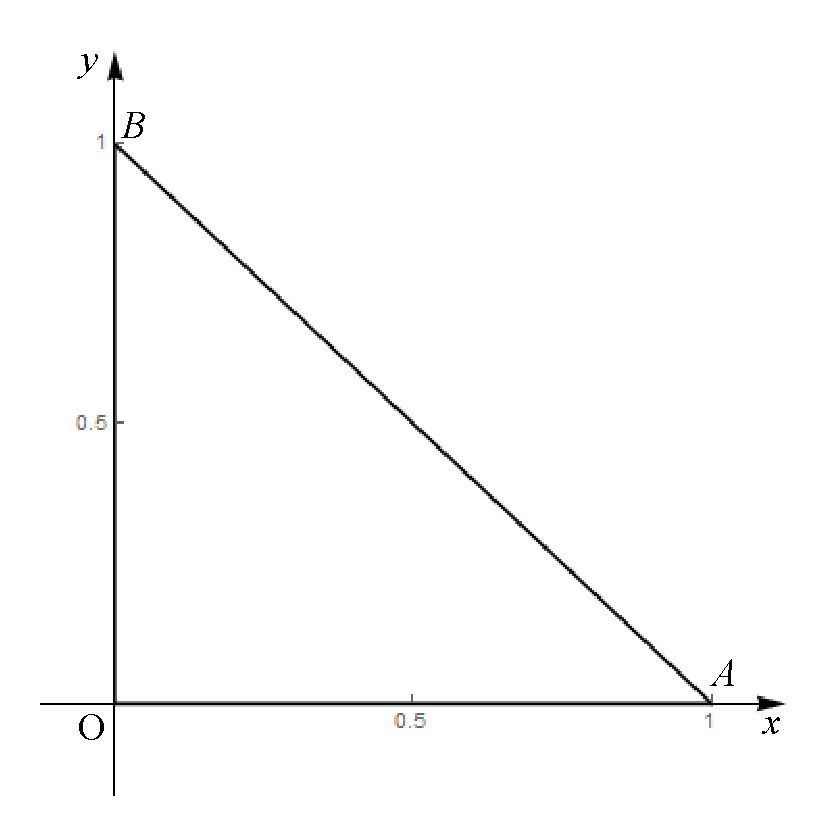
\includegraphics[height=0.3\textheight]{Figures20/Fig12-5-1.pdf}
\end{center}
\caption{习题12.5 1.题图示}
\label{12-5-1}
\end{figure}

\item计算$\LInt L{|y|}l$,其中$L$为圆心在坐标原点的右半单位圆周.

解:设$L_1$为圆心在原点的单位圆周在第一象限的部分,极坐标下的方程为$r(\theta)=1,0\leqslant\theta\leqslant\frac\pi2$,

根据对称性可知$\LInt L{|y|}l=2\LInt{L_1}yl=2\Int0{\frac\pi2}{\sin\theta\sqrt{[r(\theta)]^2+[r'(\theta)]^2}}\theta=2\Int0{\frac\pi2}{\sin\theta}\theta=2$.

\item求$\LInt L{y^2}l$,其中$L$为摆线$x=a(t-\sin t),y=a(1-\cos t)(0\leqslant t\leqslant2\pi,a>0)$的一拱.

解:$\LInt L{y^2}l=\Int0{2\pi}{a^2(1-\cos t)^2\sqrt{[x'(t)]^2+[y'(t)]^2}}t\\
=\Int0{2\pi}{a^2(1-\cos t)^2\sqrt{[a(1-\cos t)]^2+[a\sin t]^2}}t=\Int0{2\pi}{a^2(1-\cos t)^2\sqrt{a^2(2-2\cos t)}}t\\
=a^3\Int0{2\pi}{(2\sin^2\frac t2)^2\sqrt{2\cdot2\sin^2\frac t2}}t=8a^3\Int0{2\pi}{\sin^5\frac t2}t=16a^3\Int0\pi{\sin^5u}u=32a^3\Int0{\frac\pi2}{\sin^5u}u\\
=32a^3\frac{4\cdot2}{5\cdot3}=\frac{256}{15}a^3$.

{\bf注:}如图~\ref{12-5-3}所示.
\begin{figure}[H]
\begin{center}
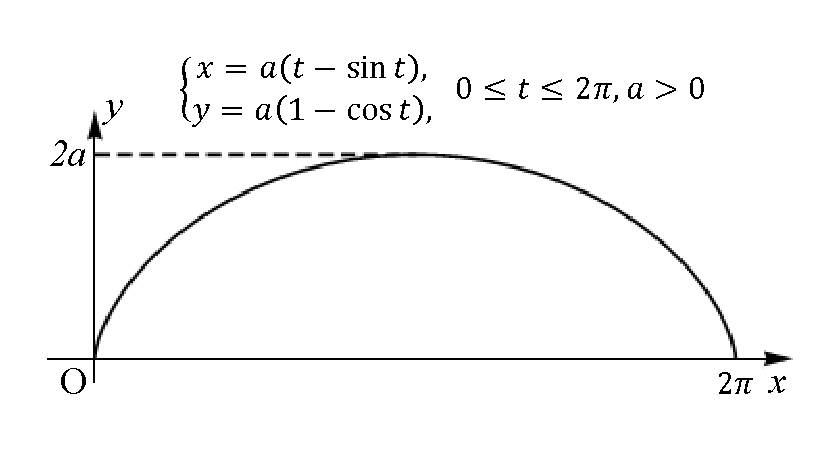
\includegraphics[height=0.2\textheight]{Figures20/Fig12-5-3.pdf}
\end{center}
\caption{习题12.5 3.题图示}
\label{12-5-3}
\end{figure}

\item计算$\LInt L{\sqrt{x^2+y^2}}l$,其中$L$为圆周$x^2+y^2=ax$.

解:$L$在极坐标下的方程为$r(\theta)=a\cos\theta,\frac\pi2\leqslant\theta\leqslant\frac\pi2$,

$\LInt L{\sqrt{x^2+y^2}}l=\Int{-\frac\pi2}{\frac\pi2}{r(\theta)\sqrt{[r(\theta)]^2+[r'(\theta)]^2}}\theta=\Int{-\frac\pi2}{\frac\pi2}{a\cos\theta\sqrt{[a\cos\theta]^2+[-a\sin\theta]^2}}\theta\\
=2a^2\Int0{\frac\pi2}{\cos\theta}\theta=2a^2$.

\item设$L$为椭圆$\frac{x^2}4+\frac{y^2}3=1$,周长为$a$,求$\varoint_L(2xy+3x^2+4y^2)\mathrm dl$.

解:根据对称性可知$\varoint_L2xy\mathrm dl=0$,

$\therefore\varoint_L(2xy+3x^2+4y^2)\mathrm dl=\varoint_L(3x^2+4y^2)\mathrm dl=12\varoint_L(\frac{x^2}4+\frac{y^2}3)\mathrm dl=12\varoint_L\mathrm dl=12a$.

\item设曲线为$\begin{cases}
x=\mathrm e^{-t}\cos t,\\
y=\mathrm e^{-t}\sin t,\\
z=\mathrm e^{-t},
\end{cases}0<t<+\infty$,求曲线的弧长.

解:记该曲线为$L$,其弧长为

$\LInt L{}l=\Int0{+\infty}{\sqrt{[x'(t)]^2+[y'(t)]^2+[z'(t)]^2}}t\\
=\Int0{+\infty}{\sqrt{[-\mathrm e^{-t}(\cos t+\sin t)]^2+[-\mathrm e^{-t}(\sin t-\cos t)]^2+[-\mathrm e^{-t}]^2}}t\\
=\Int0{+\infty}{\mathrm e^{-t}\sqrt{(\cos t+\sin t)^2+(\sin t-\cos t)^2+1}}t=\Int0{+\infty}{\mathrm e^{-t}\sqrt3}t=-\sqrt3\mathrm e^{-t}\big|_0^{+\infty}=\sqrt3$.

{\bf注:}如图~\ref{12-5-6}所示.
\begin{figure}[H]
\begin{center}
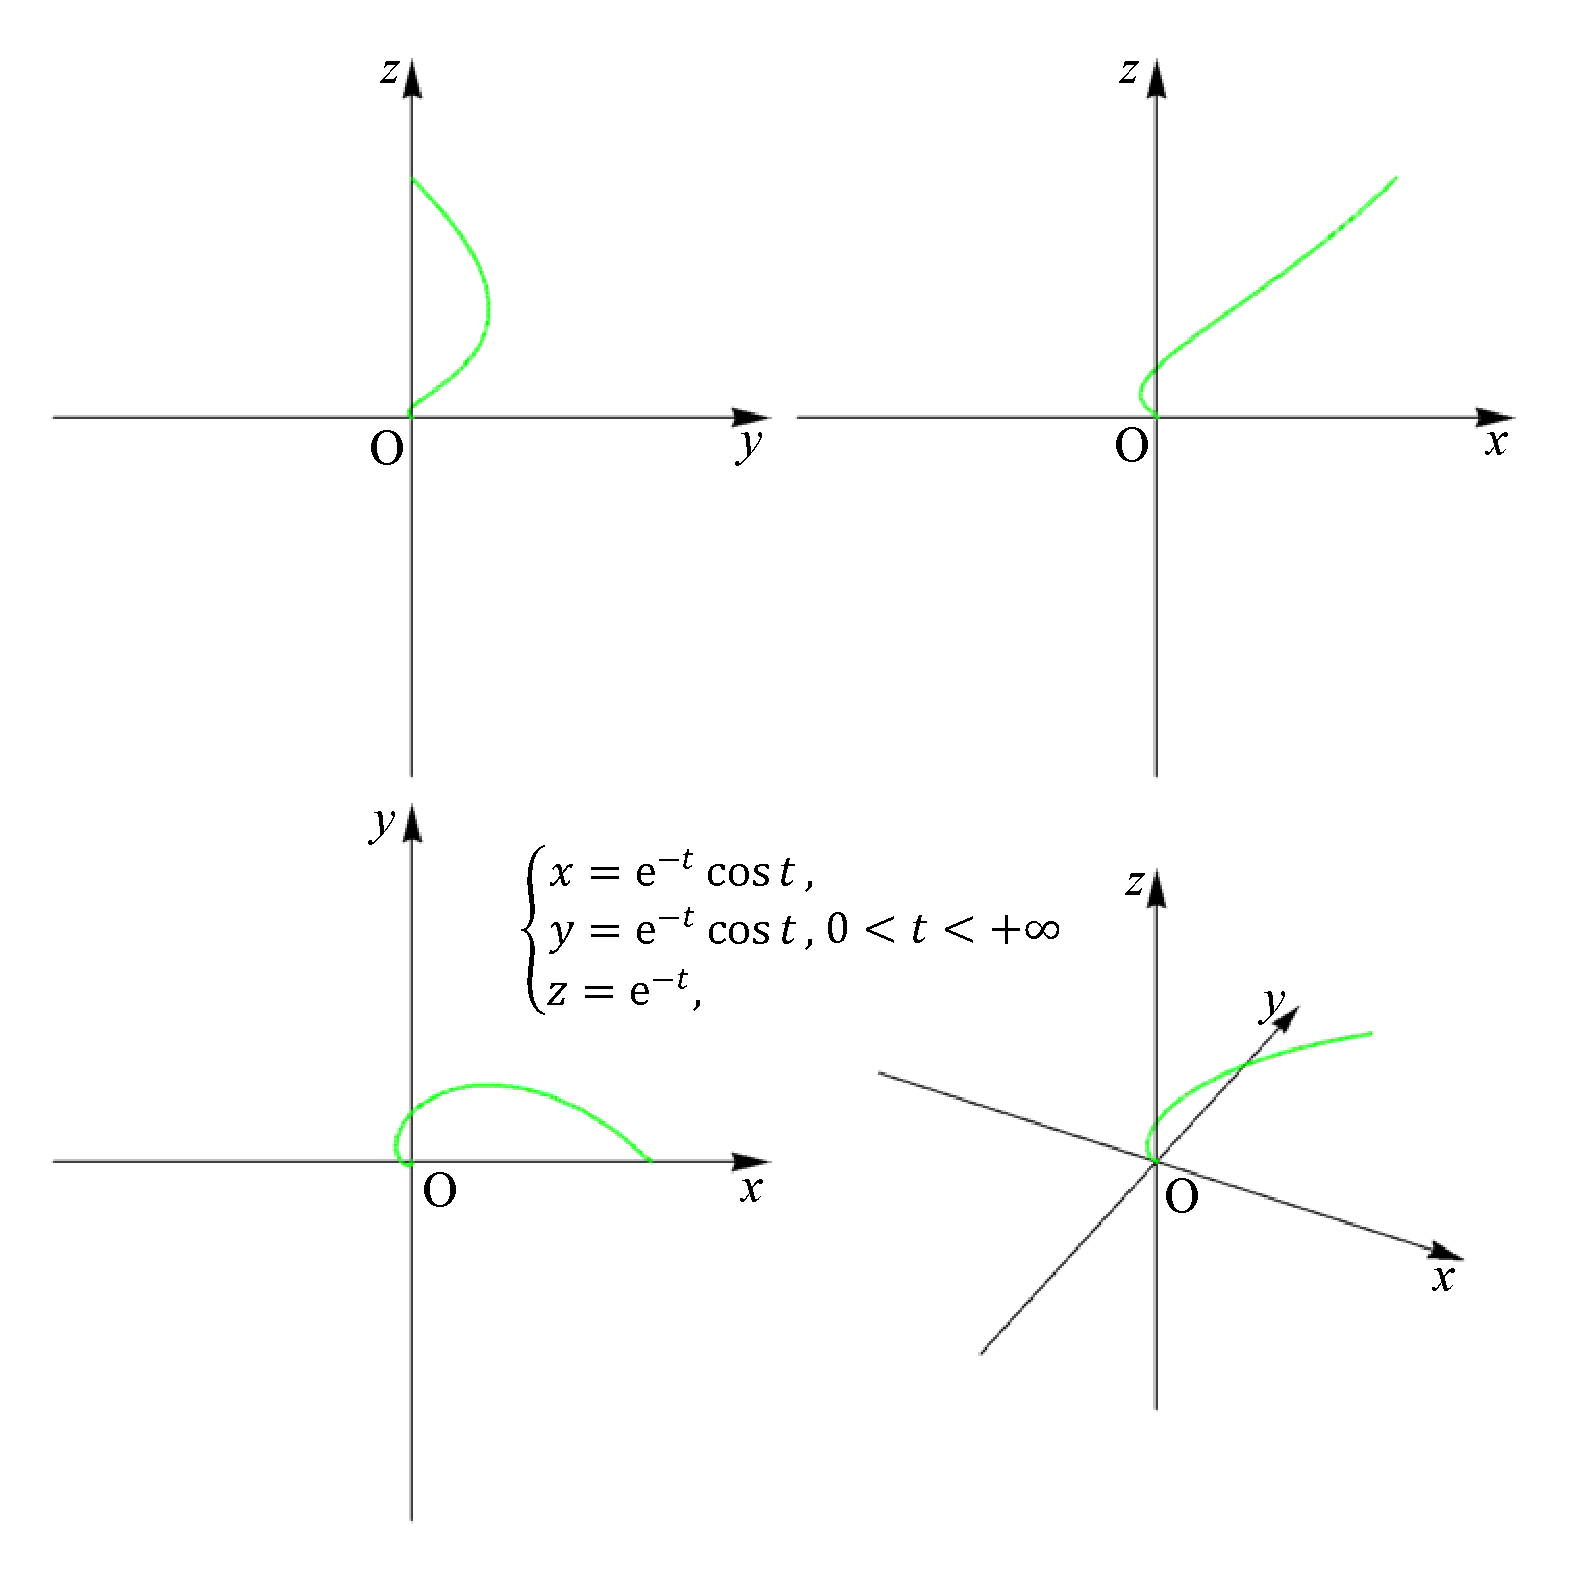
\includegraphics[height=0.7\textheight]{Figures20/Fig12-5-6.pdf}
\end{center}
\caption{习题12.5 6.题图示}
\label{12-5-6}
\end{figure}

\item计算$\LInt L{(x^2+y^2+z^2)}l$,其中$L$为螺旋线$x=a\cos t,y=a\sin t,z=bt(0\leqslant t\leqslant2\pi)$的一段.

解:$\LInt L{(x^2+y^2+z^2)}l=\Int0{2\pi}{(a^2\cos^2t+a^2\sin^2t+b^2t^2)\sqrt{[-a\sin t]^2+[a\cos t]^2+b^2}}t\\
=\sqrt{a^2+b^2}\Int0{2\pi}{(a^2+b^2t^2)}t=\sqrt{a^2+b^2}(a^2t+\frac13b^2t^3)\big|_0^{2\pi}=(2\pi a^2+\frac83\pi^3b^2)\sqrt{a^2+b^2}$.

{\bf注:}如图~\ref{12-5-7}所示.
\begin{figure}[H]
\begin{center}
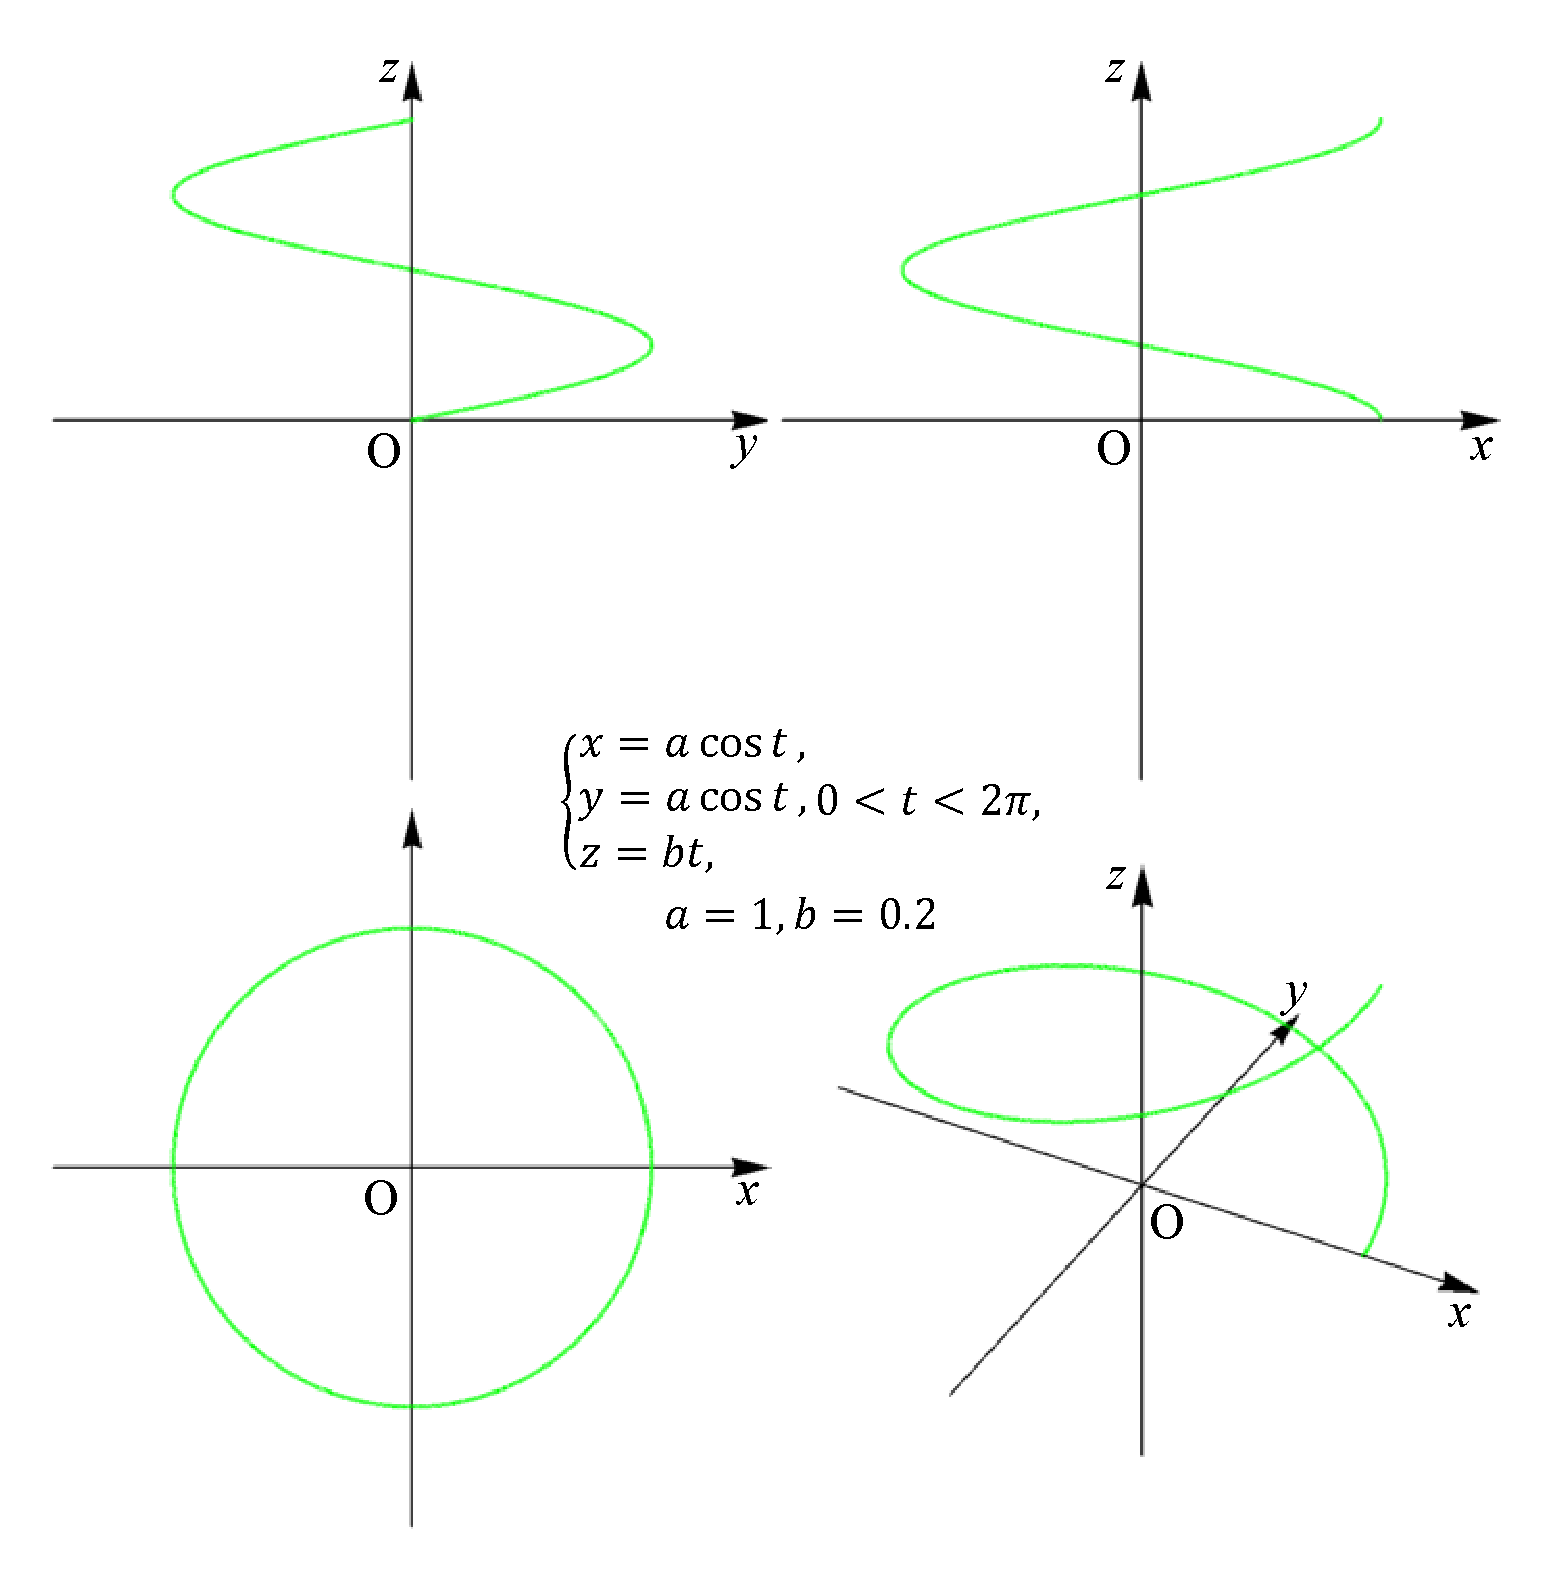
\includegraphics[height=0.7\textheight]{Figures20/Fig12-5-7.pdf}
\end{center}
\caption{习题12.5 7.题图示}
\label{12-5-7}
\end{figure}
\end{enumerate}
\subsection{习题12.6解答}
\begin{enumerate}
\item求锥面$z=\sqrt{x^2+y^2}$在柱面$z^2=2x$内的部分面积.

解:将$z=\sqrt{x^2+y^2}$代入$z^2=2x$得锥面和柱面的交线所在的投影柱面为$x^2+y^2=2x$,记锥面在柱面内的部分为$\Sigma$,$\Sigma$在$xOy$平面内的投影为圆形区域$D=\Set{(x,y)}{x^2+y^2\leqslant2x}$,

$\Sigma$的面积$\SIInt\Sigma{}S=\varIInt{D}{\sqrt{1+(\frac{\partial z}{\partial x})^2+(\frac{\partial z}{\partial y})^2}}xy=\varIInt{D}{\sqrt{1+(\frac x{\sqrt{x^2+y^2}})^2+(\frac y{\sqrt{x^2+y^2}})^2}}xy\\
=\sqrt2\varIInt{D}{}xy=\sqrt2\pi$.

{\bf注:}如图~\ref{12-6-1}所示.
\begin{figure}[H]
\begin{center}
\subfigure[]{\label{12-6-1-1}{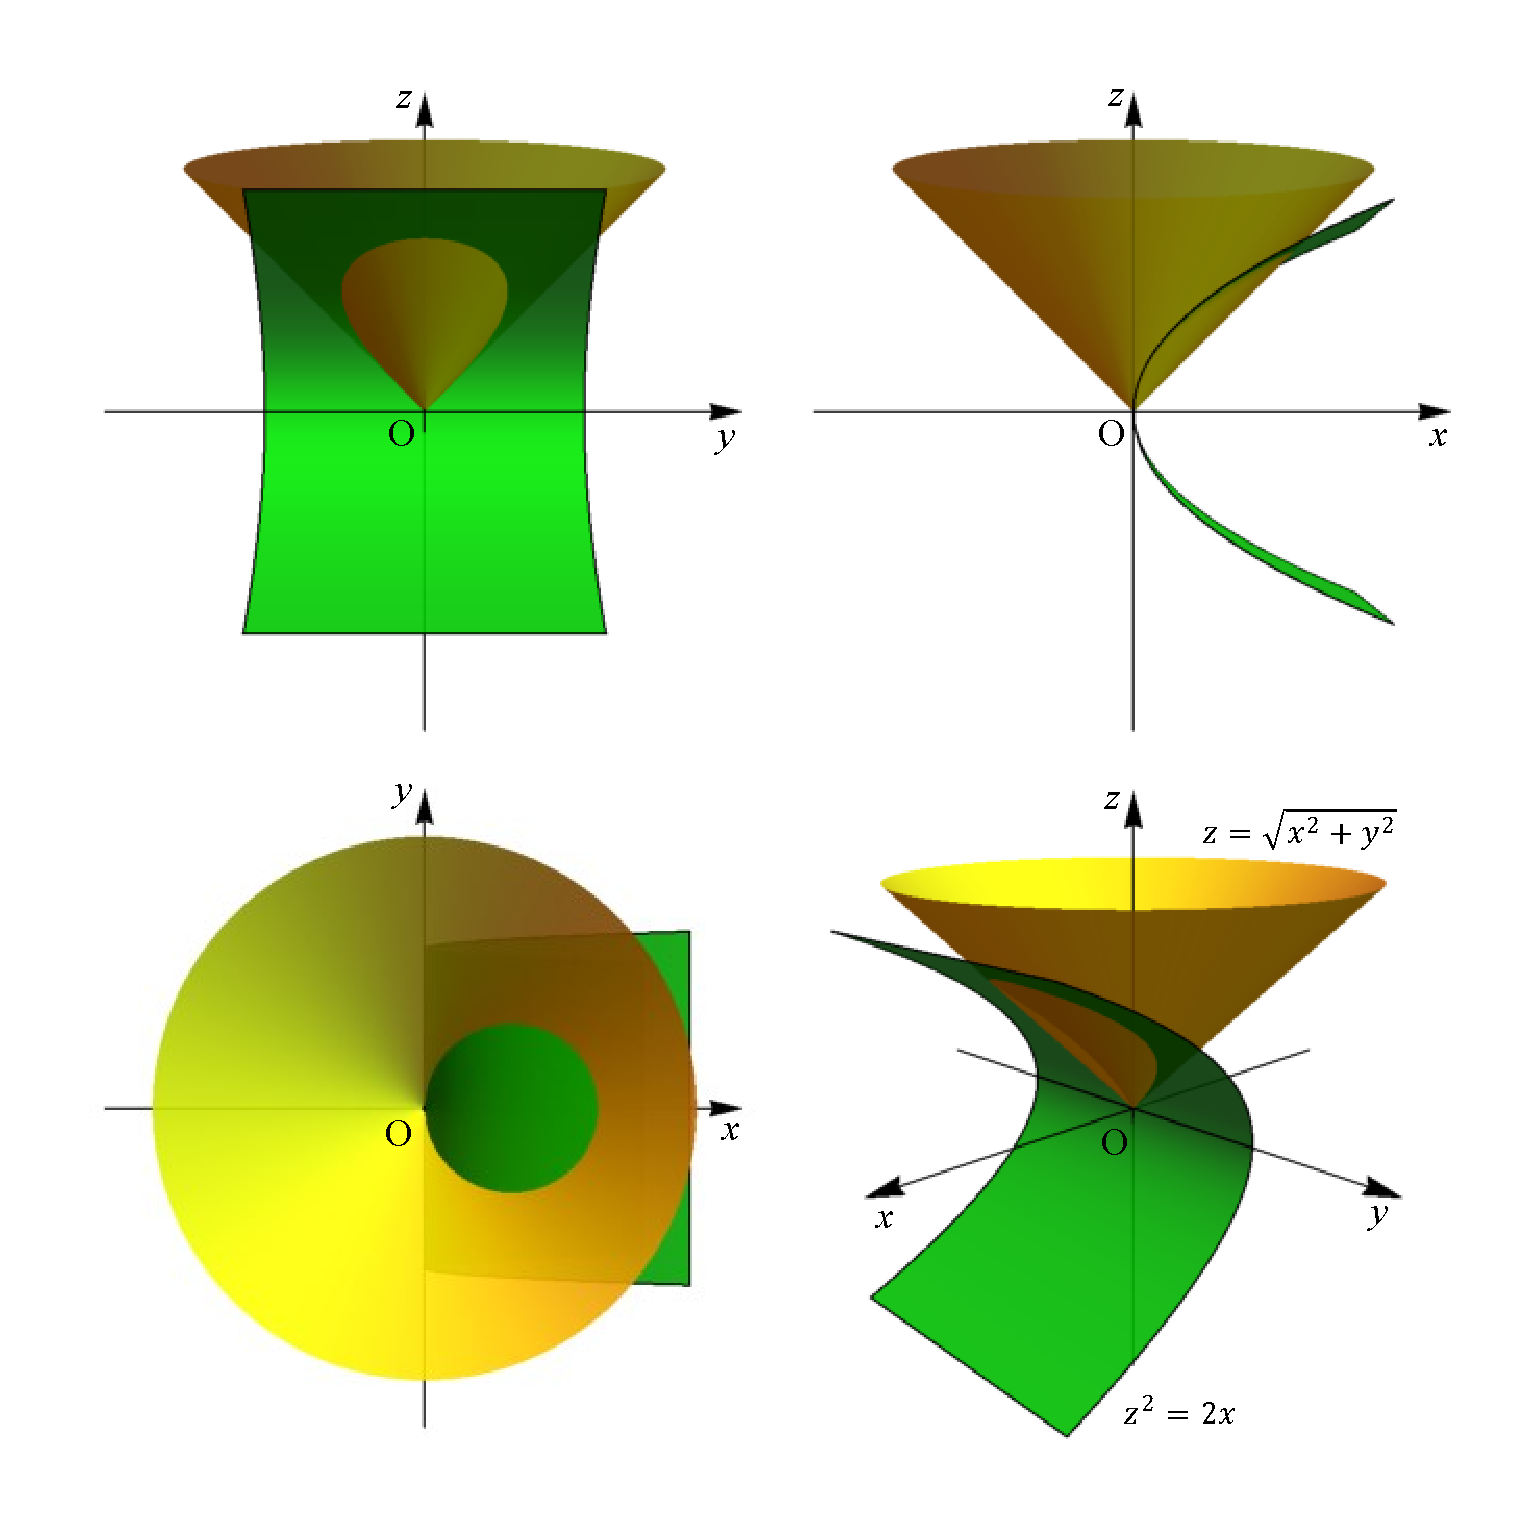
\includegraphics[height=0.68\textheight]{Figures20/Fig12-6-1-1.pdf} }}
\end{center}
\end{figure}
\addtocounter{figure}{-1}
\begin{figure}[H]
\addtocounter{figure}{1}
\begin{center}
\subfigure[]{\label{12-6-1-2} {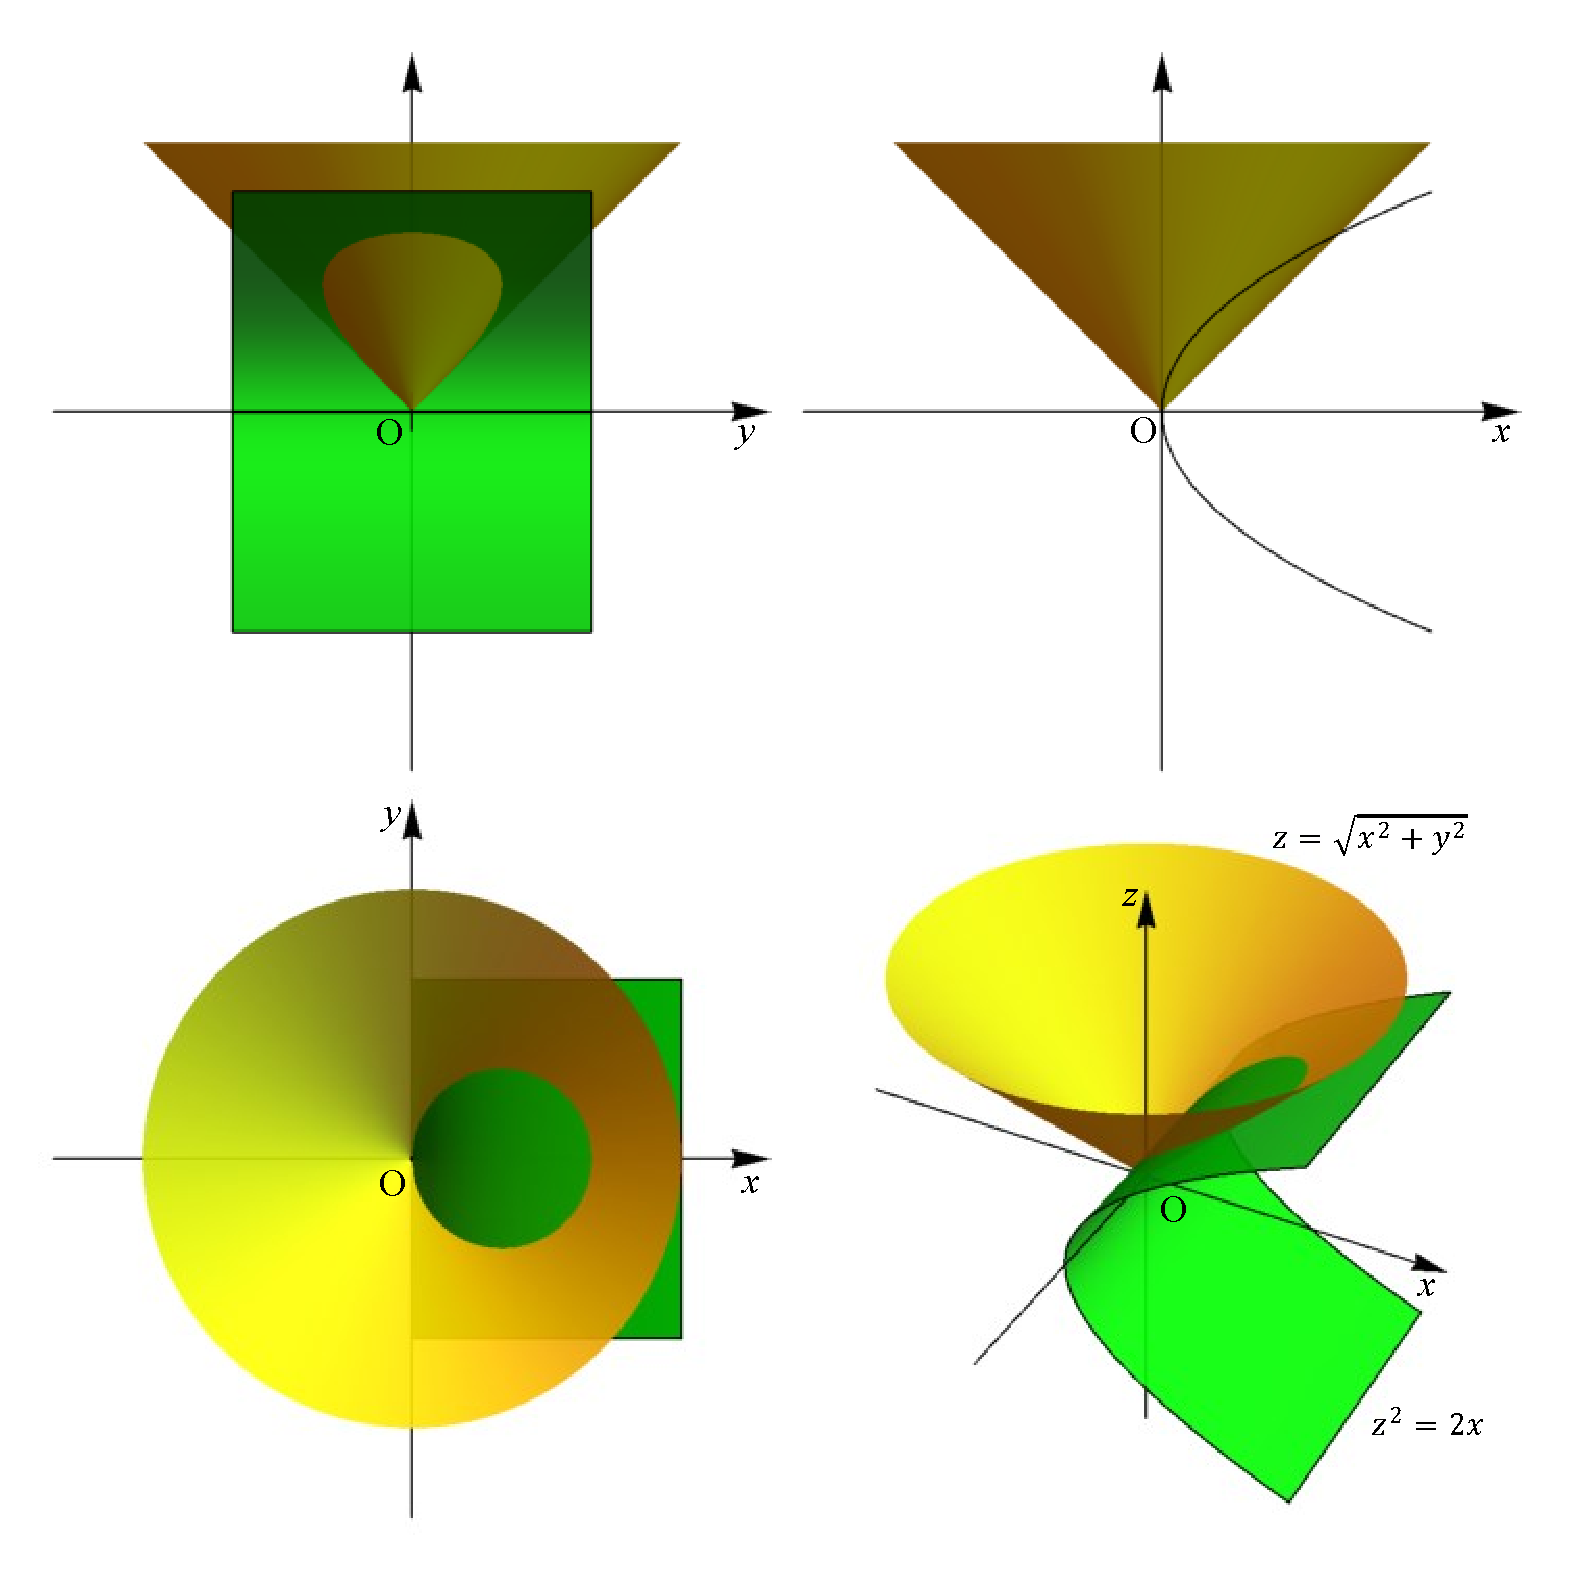
\includegraphics[height=0.70\textheight]{Figures20/Fig12-6-1-2.pdf} }}
\end{center}
\caption{习题12.6 1.题图示}
\label{12-6-1}
\end{figure}

\item求旋转抛物面$2z=x^2+y^2$被圆柱面$x^2+y^2=1$截下部分的面积.

解:记被截部分曲面为$\Sigma$,$\Sigma$在$xOy$平面上的投影域$D=\Set{(x,y)}{x^2+y^2\leqslant1}$,

$\Sigma$的面积$\SIInt\Sigma{}S=\varIInt D{\sqrt{1+(\frac{\partial z}{\partial x})^2+(\frac{\partial z}{\partial y})^2}}xy=\varIInt D{\sqrt{1+(x)^2+(y)^2}}xy=\Int0{2\pi}{}\theta\Int01{\sqrt{1+r^2}\cdot r}r\\
=2\pi\cdot\frac12\Int01{\sqrt{1+r^2}}{(1+r^2)}=\pi\frac{1}{1+\frac12}(1+r^2)^{1+\frac12}\big|_0^1=\frac23\pi(2\sqrt2-1)$.

{\bf注:}如图~\ref{12-6-2}所示.
\begin{figure}[H]
\begin{center}
\subfigure[]{\label{12-6-2-1}{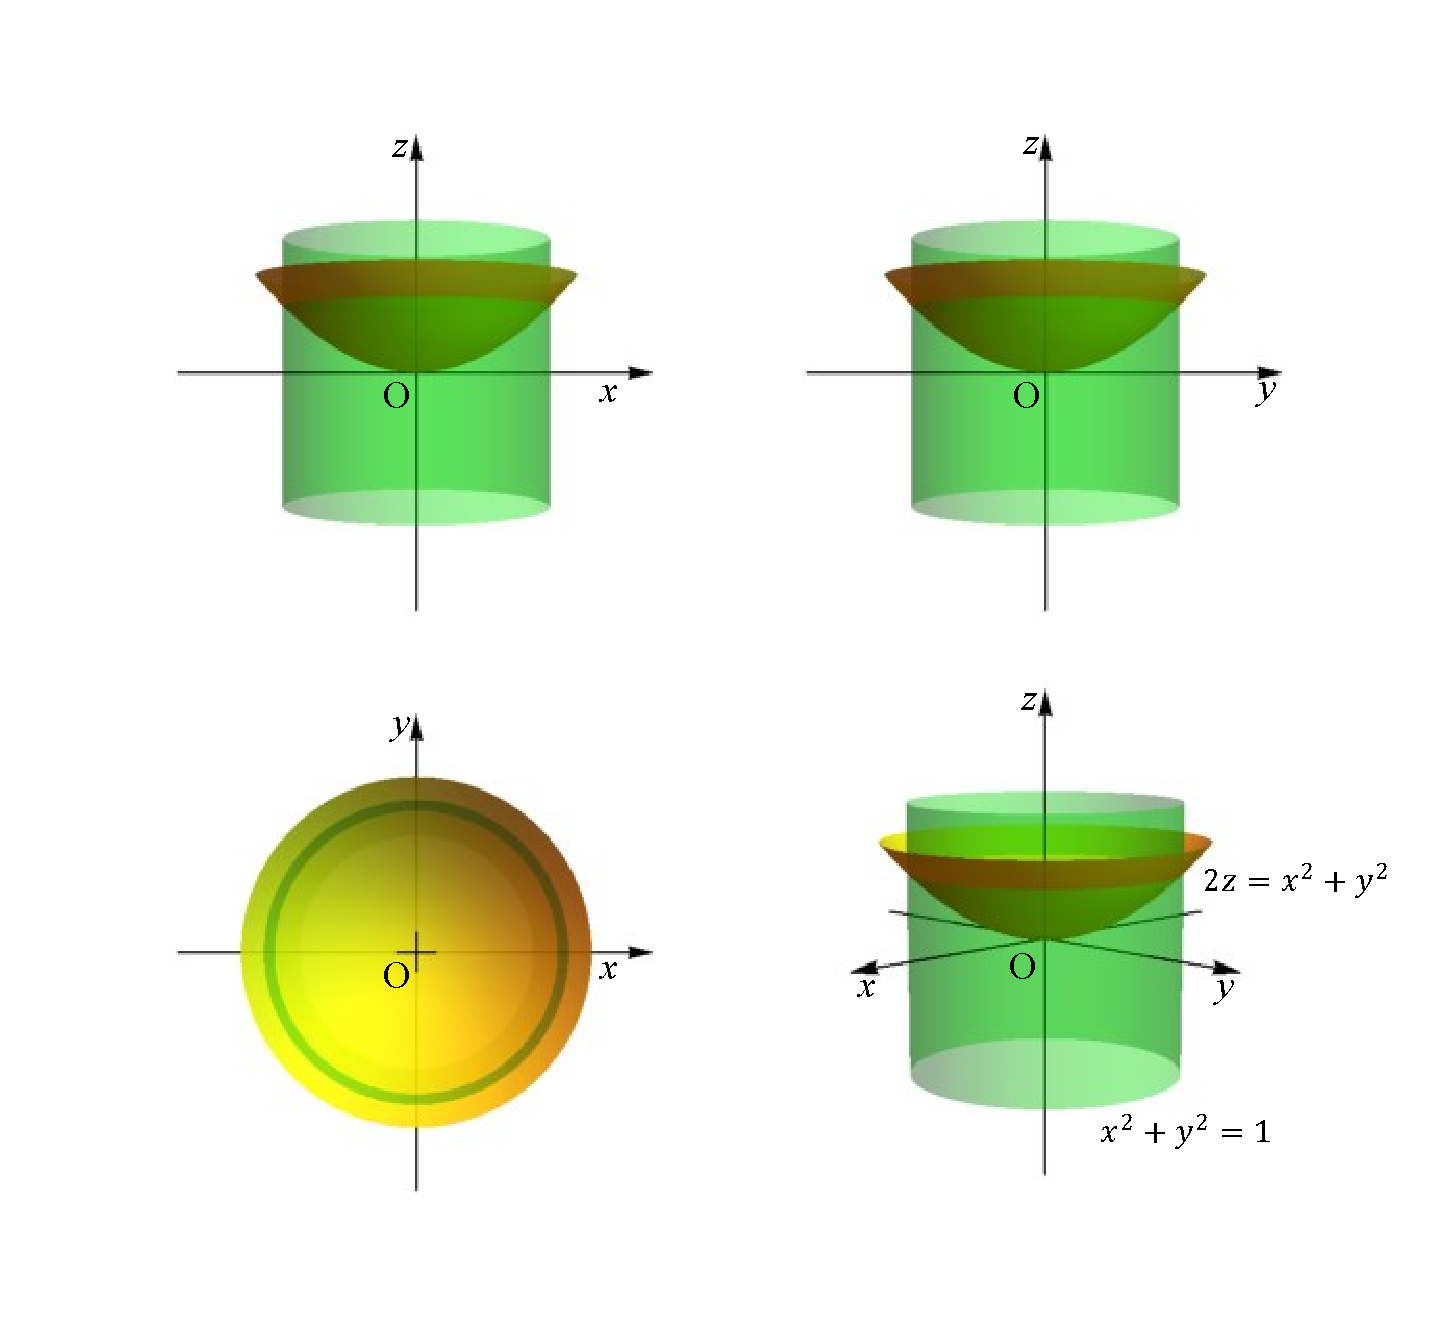
\includegraphics[height=0.68\textheight]{Figures20/Fig12-6-2-1.pdf} }}
\end{center}
\end{figure}
\addtocounter{figure}{-1}
\begin{figure}[H]
\addtocounter{figure}{1}
\begin{center}
\subfigure[]{\label{12-6-2-2} {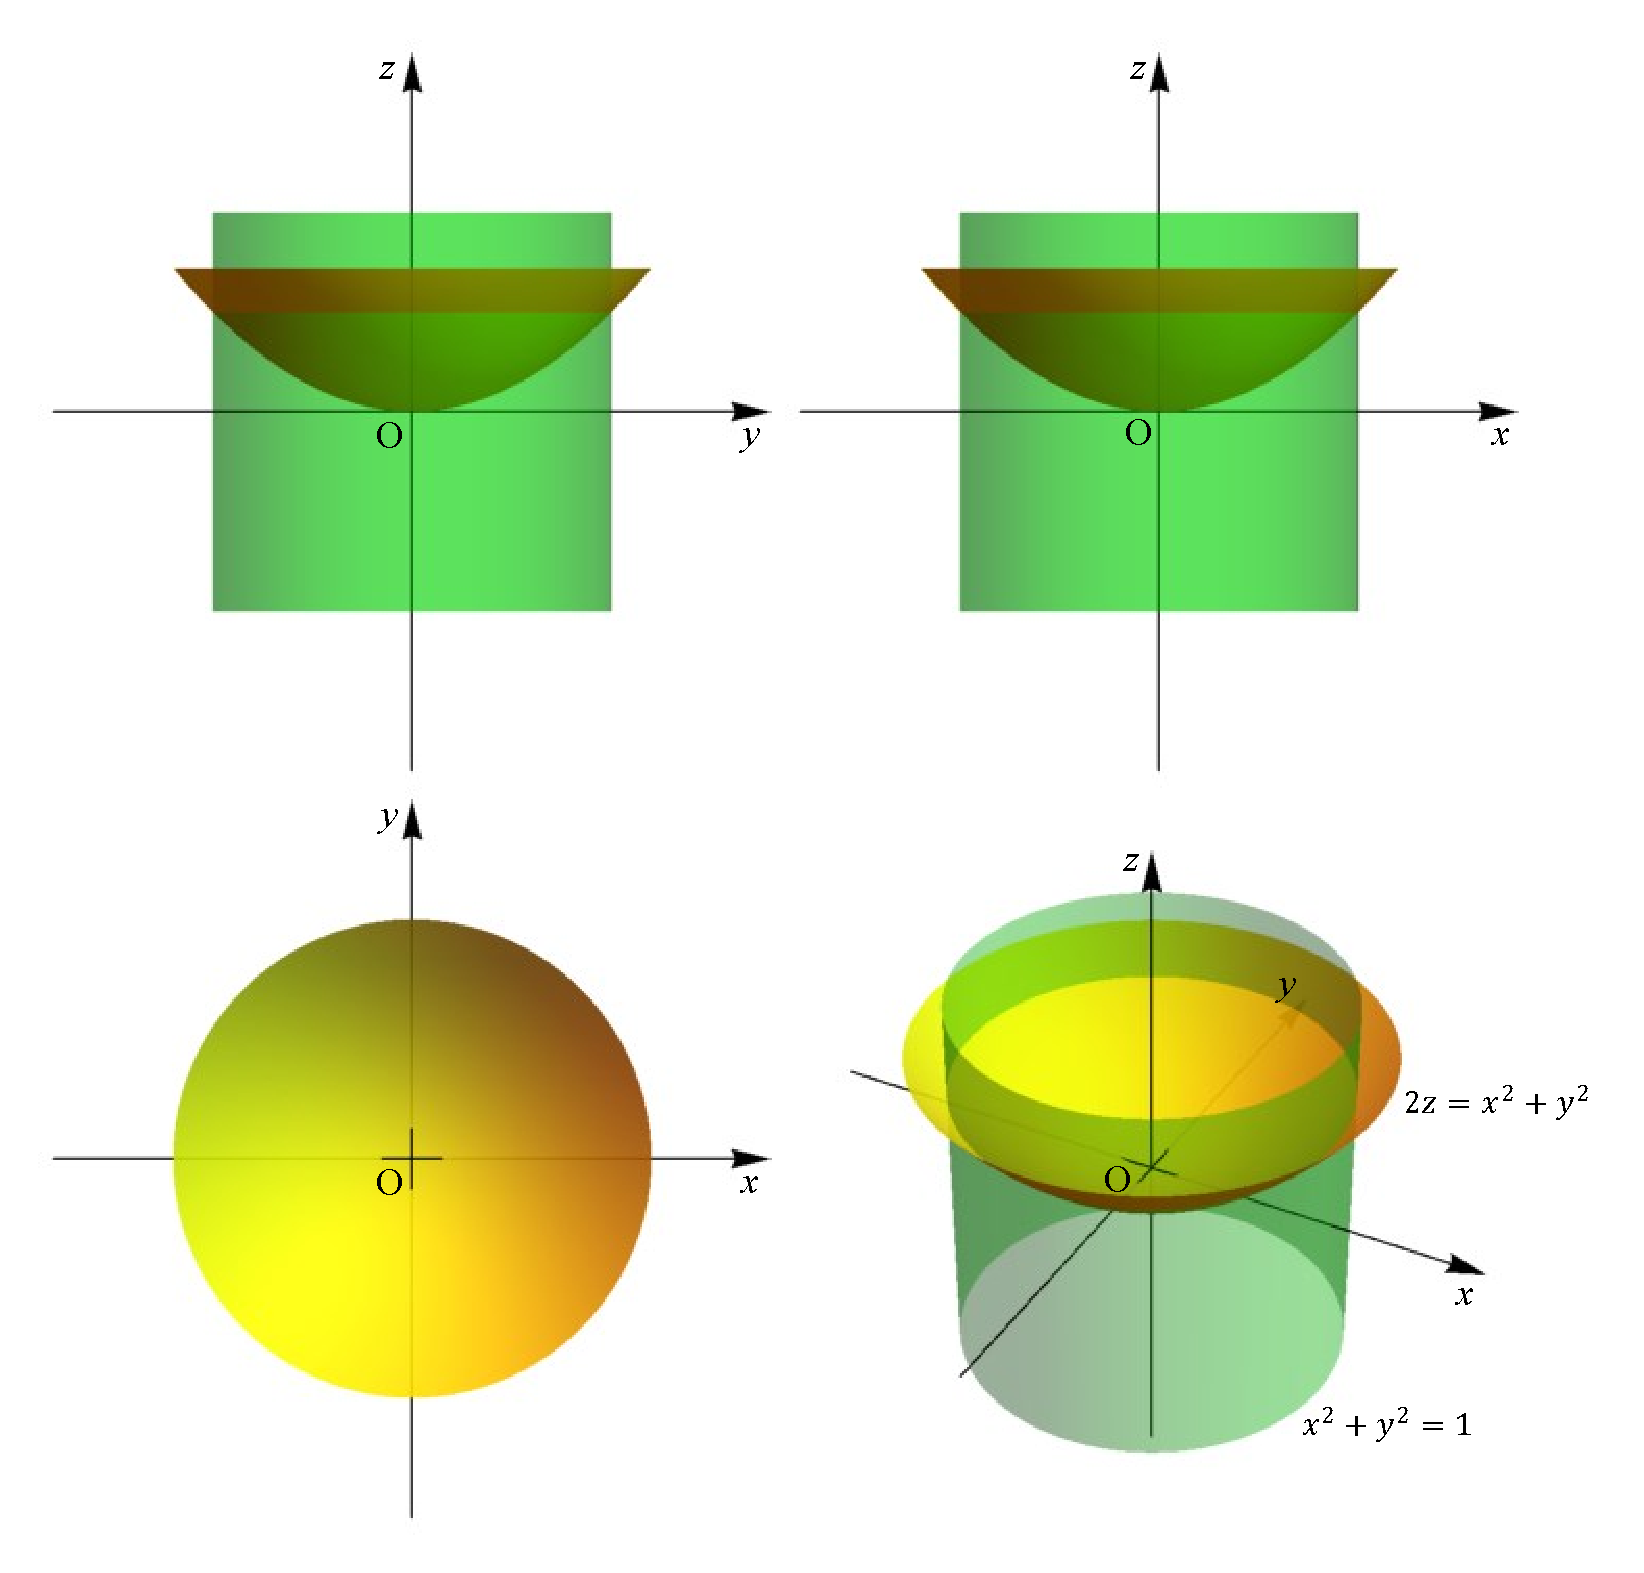
\includegraphics[height=0.70\textheight]{Figures20/Fig12-6-2-2.pdf} }}
\end{center}
\caption{习题12.6 2.题图示}
\label{12-6-2}
\end{figure}

\item求双曲抛物面$z=xy$被圆柱面$x^2+y^2=a^2$截下部分的面积.

解:记被截部分为$\Sigma$,$\Sigma$在$xOy$平面上的投影域$D=\Set{(x,y)}{x^2+y^2\leqslant a^2}$,

$\Sigma$的面积$\SIInt\Sigma{}S=\varIInt D{\sqrt{1+(\frac{\partial z}{\partial x})^2+(\frac{\partial z}{\partial y})^2}}xy=\varIInt D{\sqrt{1+(y)^2+(x)^2}}xy\\
=\Int0{2\pi}{}\theta\Int0a{\sqrt{1+r^2}\cdot r}r=\pi\frac{1}{1+\frac12}(1+r^2)^{1+\frac12}\big|_0^a=\frac23\pi[(1+a^2)^{\frac32}-1]$.

{\bf注:}如图~\ref{12-6-3-1}所示.
\begin{figure}[H]
\begin{center}
\subfigure[]{\label{12-6-3-0}{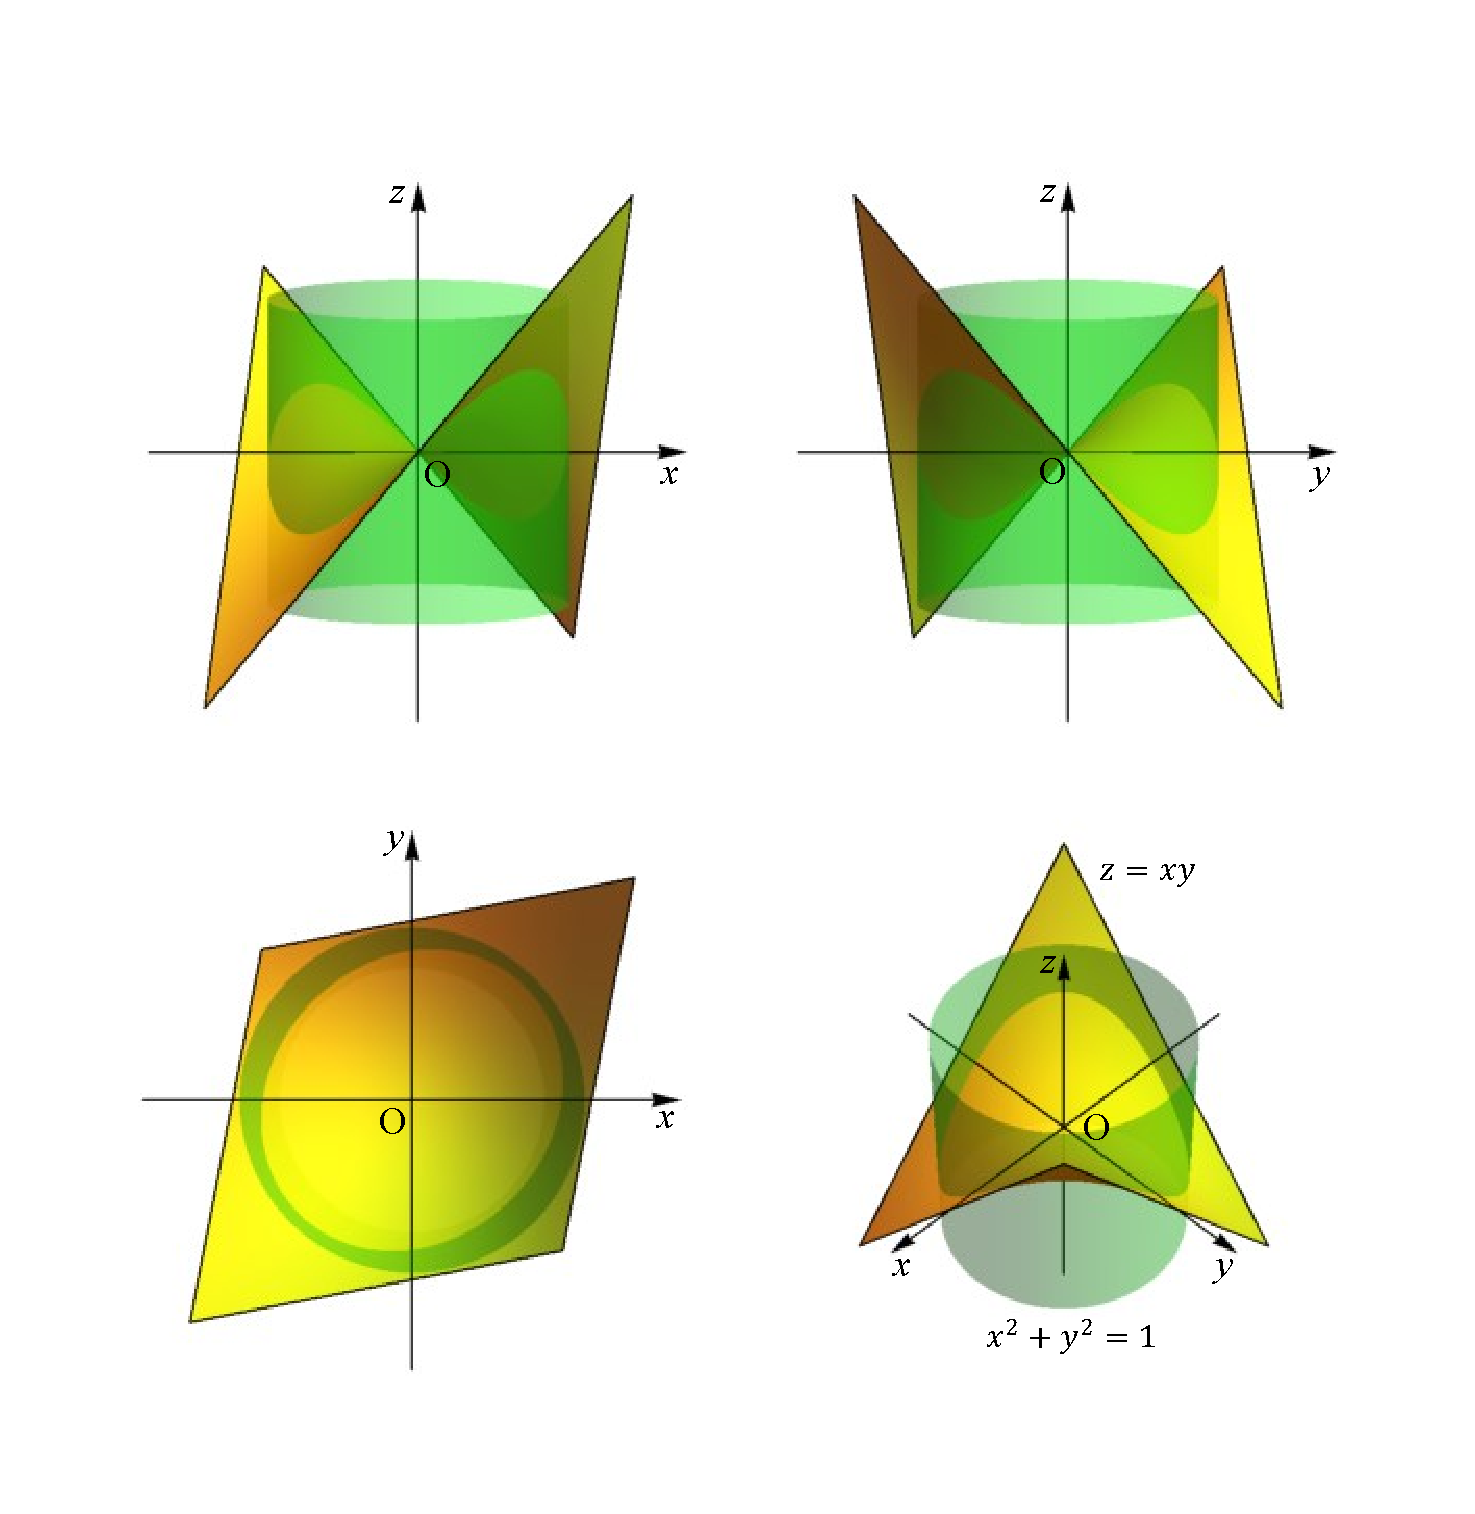
\includegraphics[height=0.75\textheight]{Figures20/Fig12-6-3-0.pdf} }}
\end{center}
\end{figure}
\addtocounter{figure}{-1}
\begin{figure}[H]
\addtocounter{figure}{1}
\begin{center}
\subfigure[]{\label{12-6-3-1} {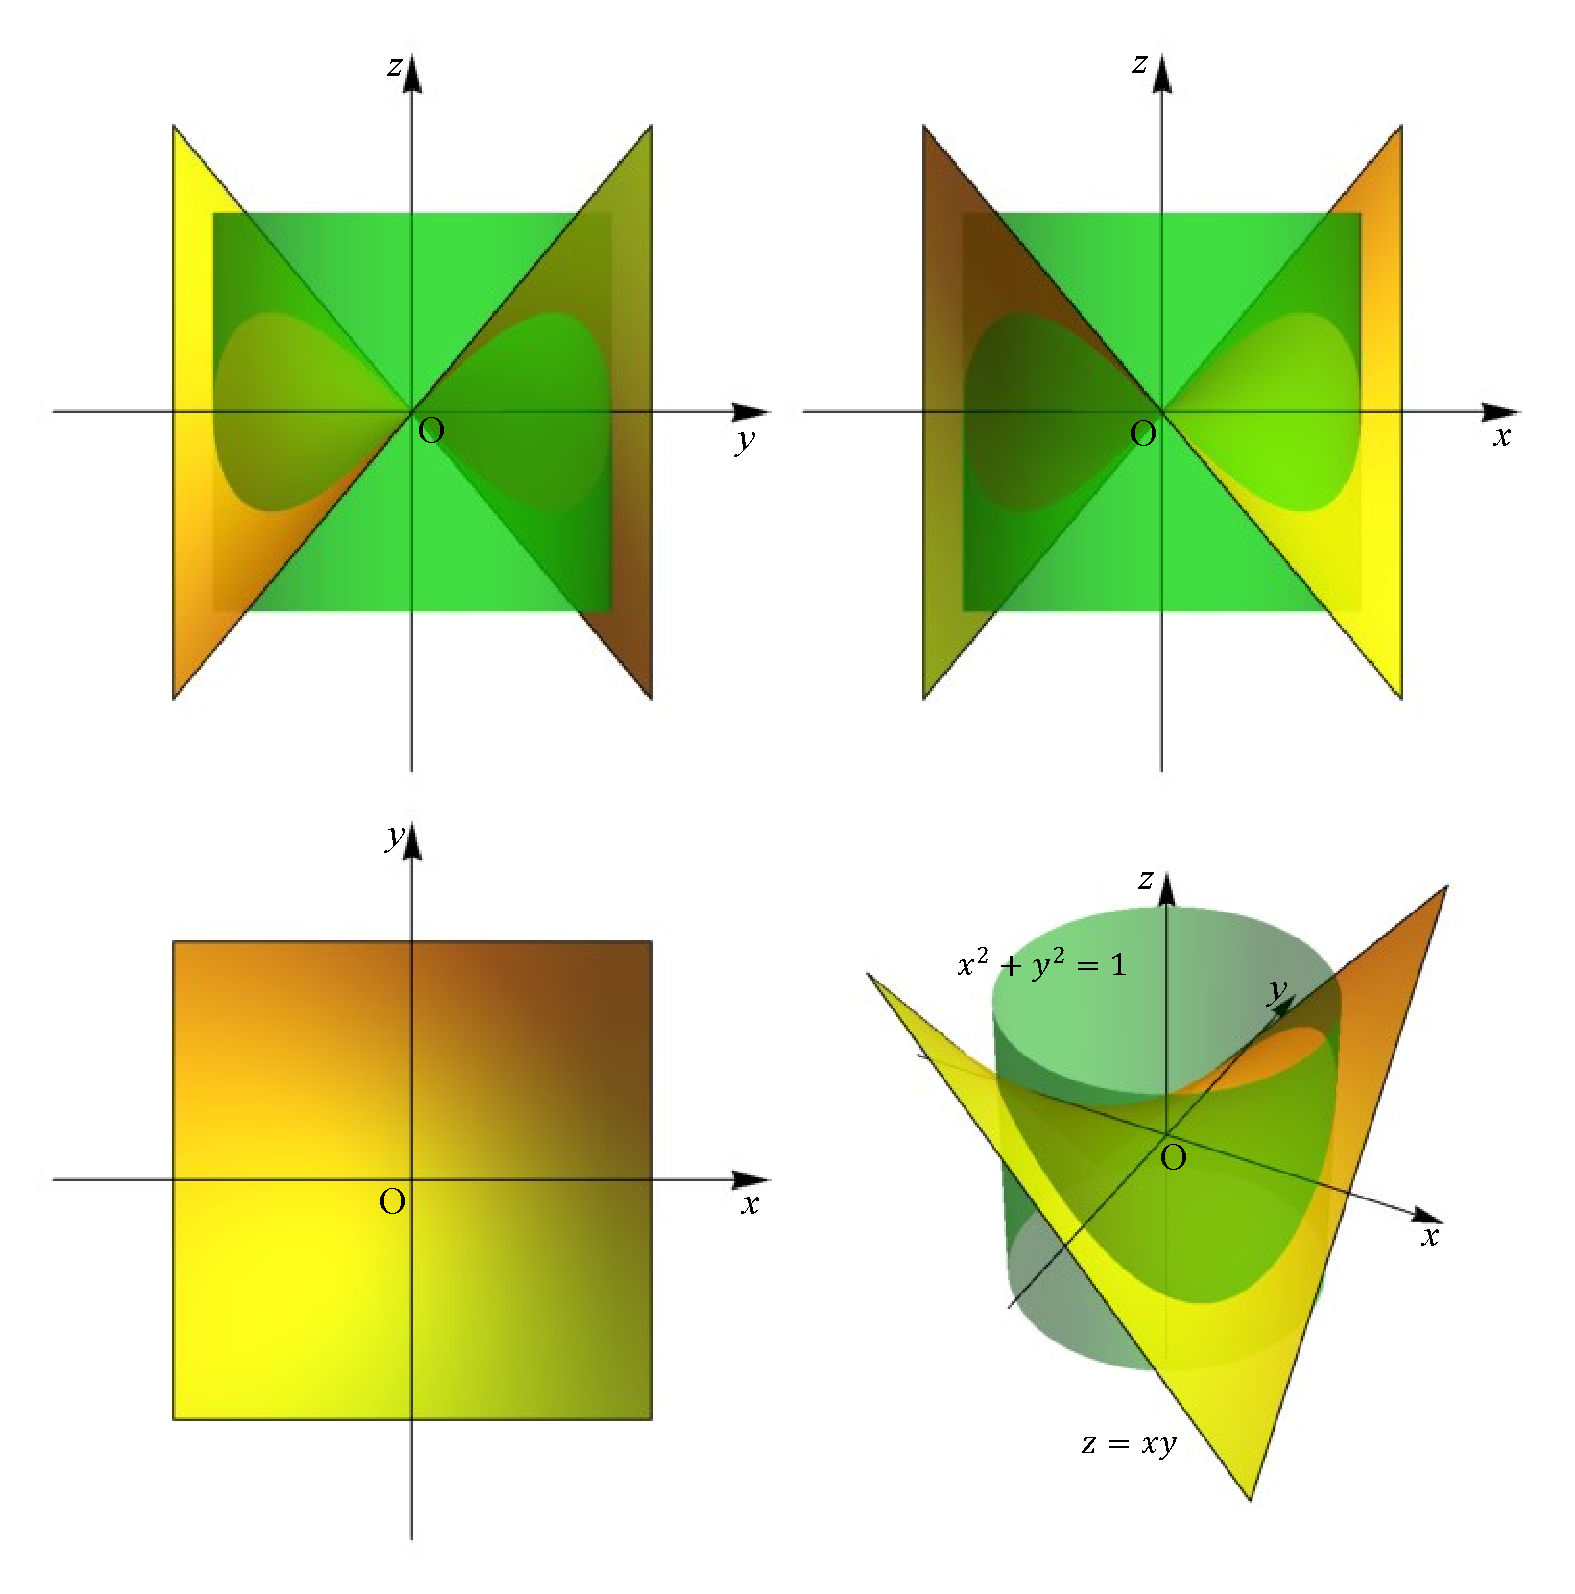
\includegraphics[height=0.70\textheight]{Figures20/Fig12-6-3-1.pdf} }}
\end{center}
\caption{习题12.6 3.题图示}
\label{12-6-3}
\end{figure}
\item计算下列第一型曲面积分:\\
(1)$\SIInt S{(x+z)}S$,$S$是半球面$x^2+y^2+z^2=R^2,x\geqslant0$;\\
(2)$\SIInt S{|y\sqrt z|}S$,其中$S$是曲面$z=x^2+y^2(z\leqslant1)$;\\
(3)$\SIInt S{(ax+by+cz+d)^2}S$,$S$是球面$x^2+y^2+z^2=R^2$.

解:(1)由对称性可知$\SIInt SzS=0$,

又$\because x\geqslant0$,

$\therefore x=\sqrt{R^2-y^2-z^2},(y,z)\in\Set{(y,z)}{y^2+z^2\leqslant R^2}$,

$\therefore\SIInt S{(x+z)}S=\SIInt SxS=\varIInt D{\sqrt{R^2-y^2-z^2}\sqrt{(\frac{\partial x}{\partial x})^2+(\frac{\partial x}{\partial y})^2+(\frac{\partial x}{\partial z})^2}}yz\\
=\varIInt D{\sqrt{R^2-y^2-z^2}\sqrt{(1+(\frac{-y}{\sqrt{R^2-y^2-z^2}})^2+(\frac{-z}{\sqrt{R^2-y^2-z^2}})^2}}yz\\
=\varIInt D{\sqrt{R^2-y^2-z^2}\frac R{\sqrt{R^2-y^2-z^2}}}yz\\
=R\varIInt D{}yz=\pi R^3$.

{\bf注:}如图~\ref{12-6-4-1}所示.
\begin{figure}[H]
\begin{center}
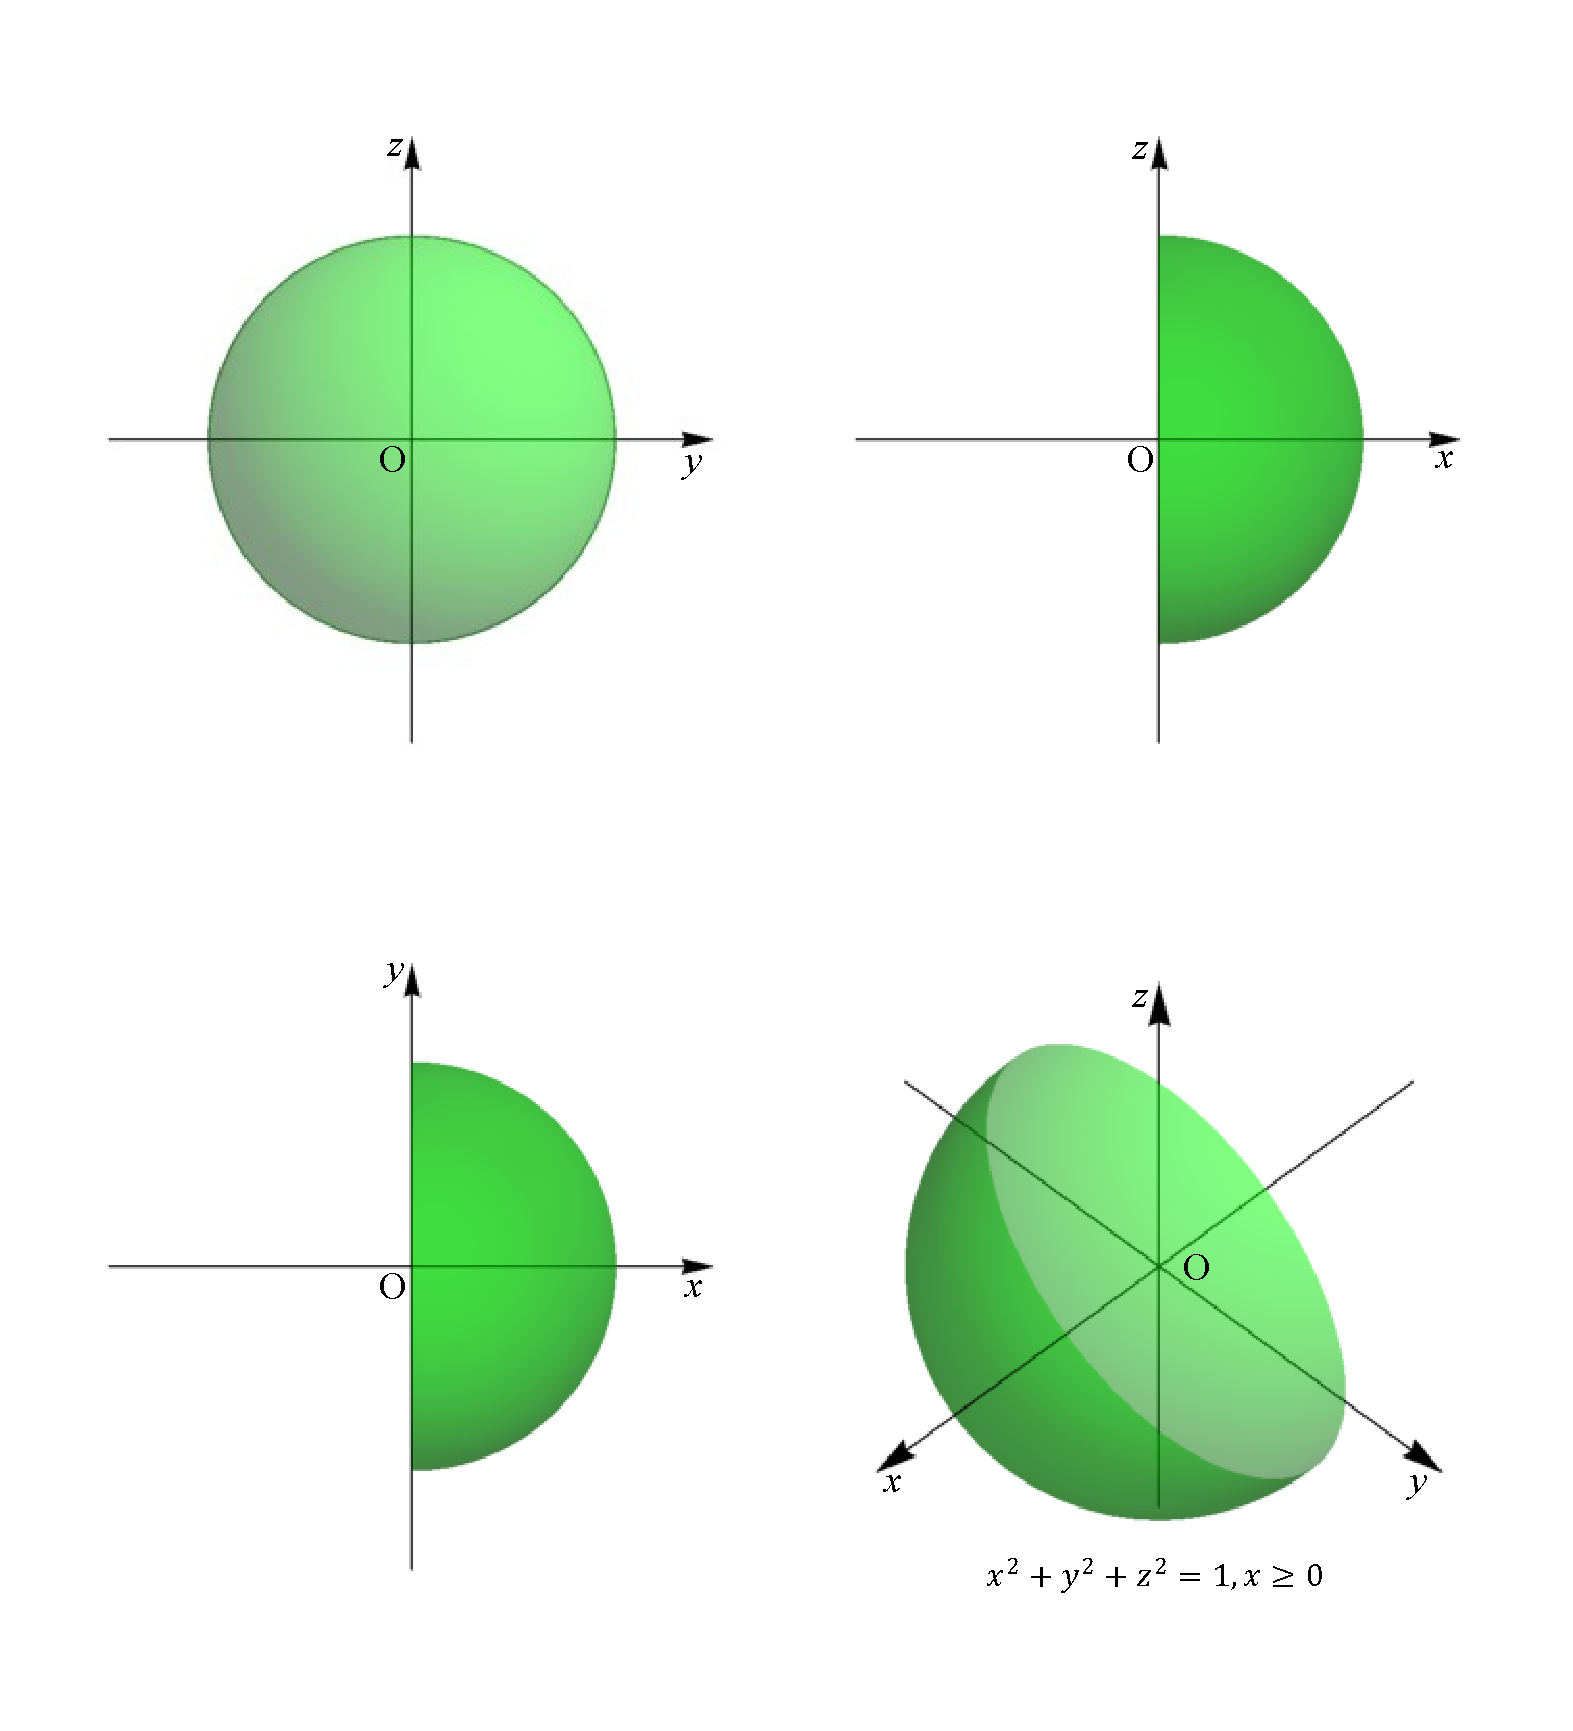
\includegraphics[height=0.75\textheight]{Figures20/Fig12-6-4-1.pdf}
\end{center}
\caption{习题12.6 4.(1)题图示}
\label{12-6-4-1}
\end{figure}

(2)由对称性可知$\SIInt S{|y\sqrt z|}S=2\SIInt{S_1}{y\sqrt z}S$,其中$S_1$是曲面$z=x^2+y^2,z\leqslant1,y\geqslant0$,$S_1$在$xOy$平面上的投影域$D=\Set{(x,y)}{x^2+y^2\leqslant1,y\geqslant0}$,

$\therefore\SIInt S{|y\sqrt z|}S=2\SIInt{S_1}{y\sqrt z}S=2\varIInt D{y\sqrt z\sqrt{1+(\frac{\partial z}{\partial x})^2+(\frac{\partial z}{\partial y})^2}}xy\\
=2\varIInt D{y\sqrt z\sqrt{1+(2x)^2+(2y)^2}}xy=2\Int0\pi{}\theta\Int01{r\sin\theta\cdot r\cdot\sqrt{1+4r^2}\cdot r}r\\
=2\Int0\pi{\sin\theta}\theta\Int01{r^3\sqrt{1+4r^2}}r=4\Int0{\frac\pi2}{\sin\theta}\theta\Int01{r^3\sqrt{1+4r^2}}r=4\Int01{r^3\sqrt{1+4r^2}}r\\
=\frac12\Int01{r^2\sqrt{1+4r^2}}{(1+4r^2)}=\frac18\Int01{(4r^2+1-1)\sqrt{1+4r^2}}{(1+4r^2)}
\\=\frac18\Int01{[(4r^2+1)^{\frac32}-\sqrt{1+4r^2}]}{(1+4r^2)}\\
=\frac18[\frac1{1+\frac32}(1+4r^2)^{\frac52}-\frac1{1+\frac12}(1+4r^2)^{\frac32}]\big|_0^1=\frac18[\frac25\cdot25\sqrt5-\frac23\cdot5\sqrt5-\frac25+\frac23]=\frac{150\sqrt5-50\sqrt5-6+10}{8\cdot15}\\
=\frac{25\sqrt5+1}{30}$.

{\bf注1:}积分法2:$4\Int01{r^3\sqrt{1+4r^2}}r\xlongequal{2r=\tan\alpha}4\Int0{\arctan2}{(\frac12\tan\alpha)^3\sqrt{1+\tan^2\alpha}}{(\frac12\tan\alpha)}\\
=\frac14\Int0{\arctan2}{\tan^3\alpha\sec\alpha\sec^2\alpha}\alpha=\frac14\Int0{\arctan2}{\tan^2\alpha\sec^2\alpha\cdot\tan\alpha\sec\alpha}\alpha\\
=\frac14\Int0{\arctan2}{(\sec^2\alpha-1)\sec^2\alpha}{\sec\alpha}=\frac14\Int0{\arctan2}{(\sec^4\alpha-\sec^2\alpha)}{\sec\alpha}\\
=\frac14(\frac15\sec^5\alpha-\frac13\sec^3\alpha)\big|_0^{\arctan2}=\frac14(\frac15\cdot25\sqrt5-\frac13\cdot5\sqrt5+\frac15-\frac13)\\
=\frac{25\sqrt5+1}{30}$.

积分法3:$4\Int01{r^3\sqrt{1+4r^2}}r=\frac12\Int01{r^2\sqrt{1+4r^2}}{(1+4r^2)}\\
=\frac12\frac1{1+\frac12}\Int01{r^2}{(1+4r^2)^{\frac32}}=\frac13[r^2(1+4r^2)^{\frac32}\big|_0^1-\Int01{(1+4r^2)^{\frac32}}{r^2}]\\
=\frac13[5\sqrt5-\frac14\Int01{(1+4r^2)^{\frac32}}{(1+4r^2)}]=\frac13[5\sqrt5-\frac14\frac1{1+\frac32}(1+4r^2)^{\frac32+1}\big|_0^1]\\
=\frac13(5\sqrt5-\frac1{10}\cdot25\sqrt5+\frac1{10})=\frac{25\sqrt5+1}{30}$.

{\bf注2:}如图~\ref{12-6-4-2}所示.
\begin{figure}[H]
\begin{center}
\subfigure[]{\label{12-6-4-2-1}{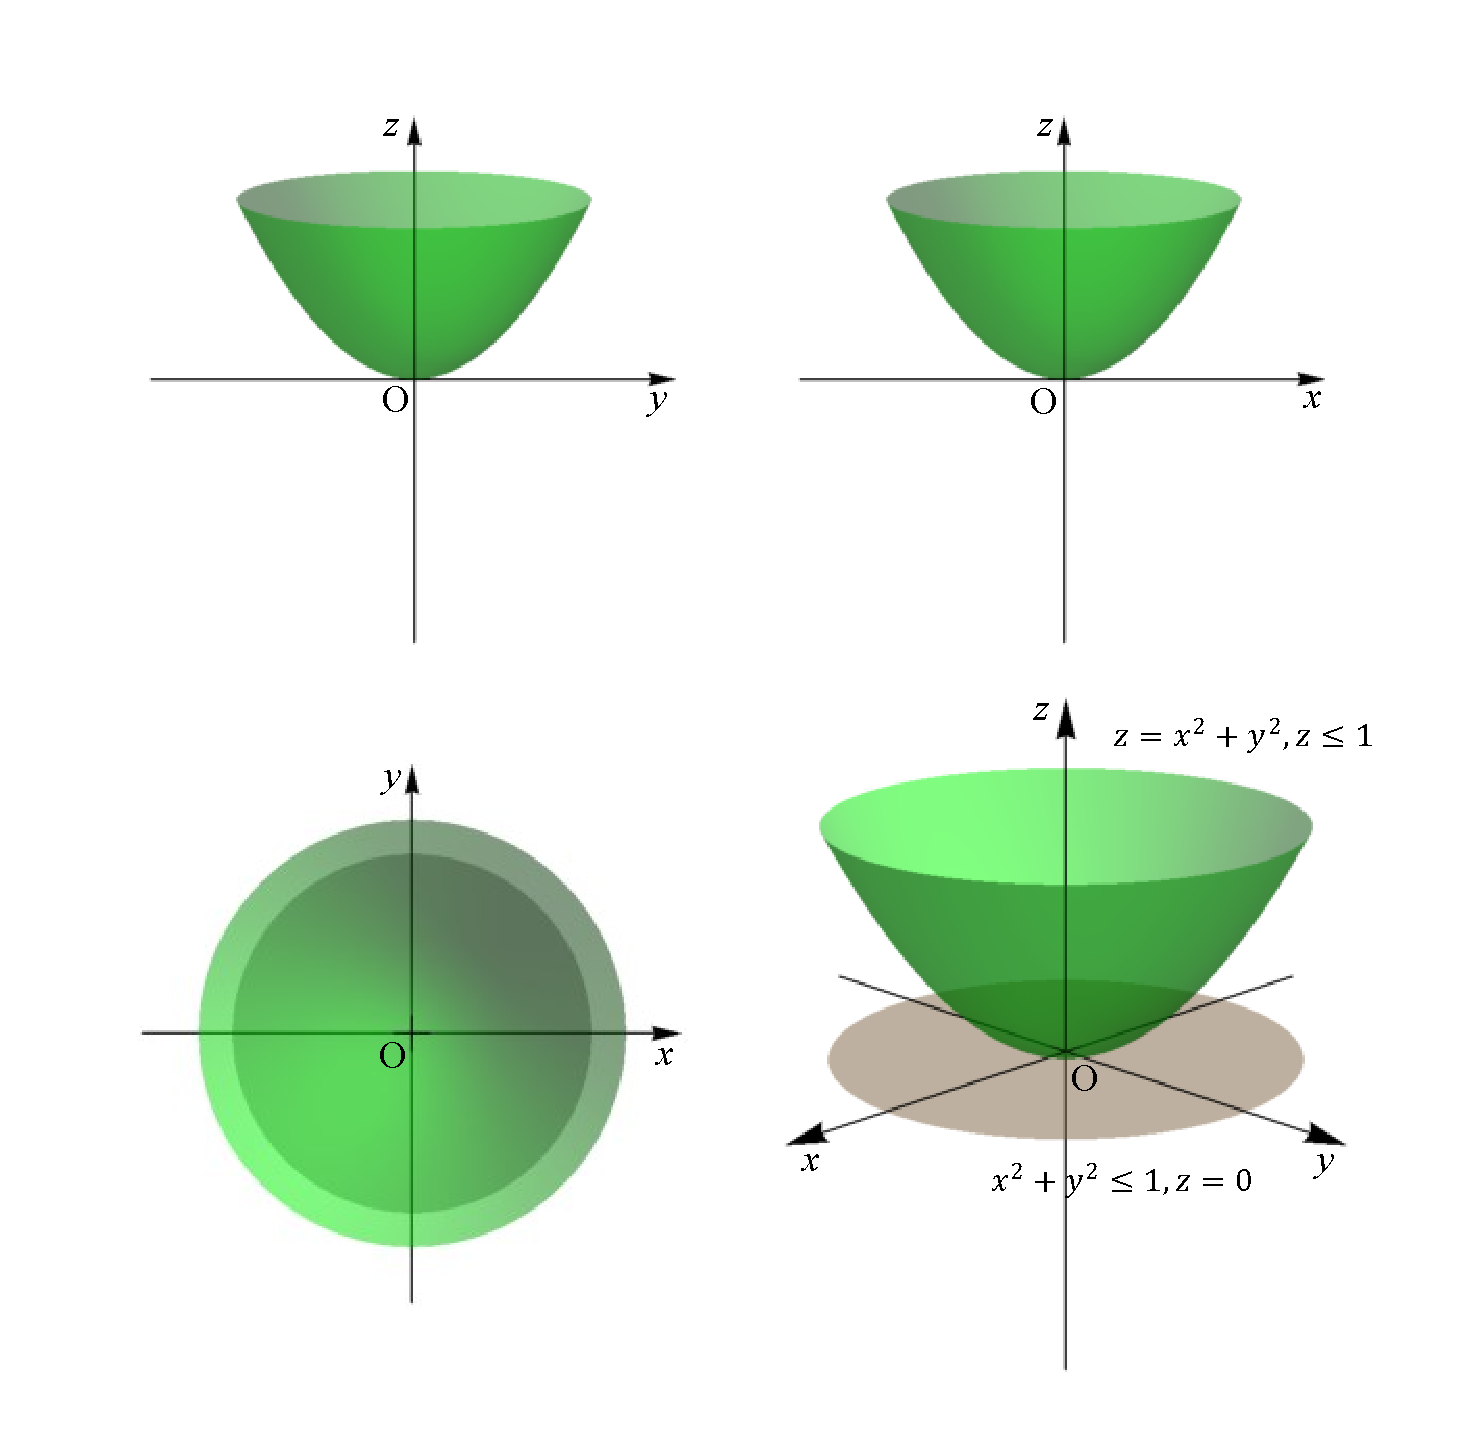
\includegraphics[height=0.70\textheight]{Figures20/Fig12-6-4-2-1.pdf} }}
\end{center}
\end{figure}
\addtocounter{figure}{-1}
\begin{figure}[H]
\addtocounter{figure}{1}
\begin{center}
\subfigure[]{\label{12-6-4-2-2} {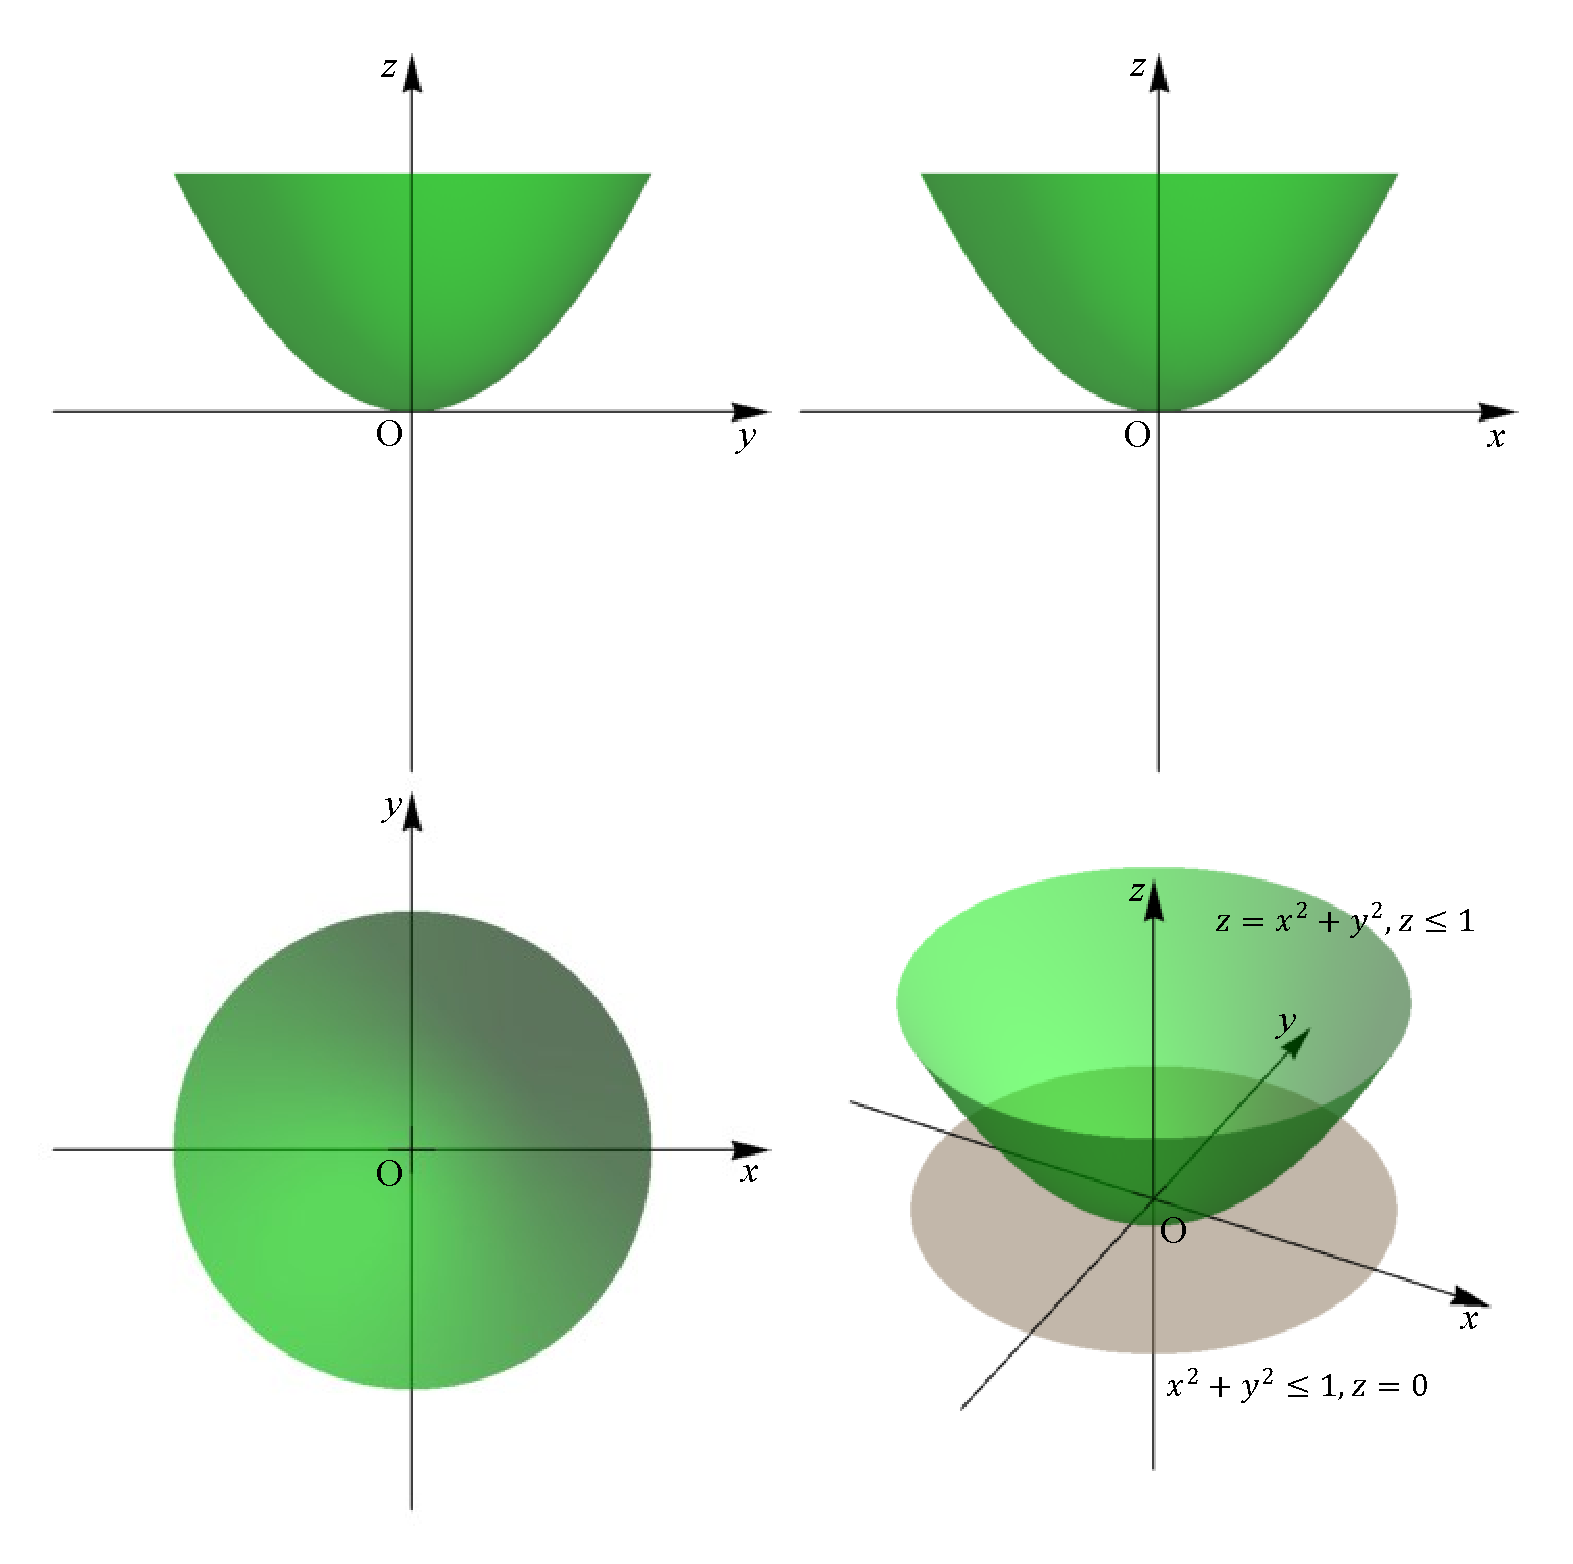
\includegraphics[height=0.70\textheight]{Figures20/Fig12-6-4-2-2.pdf} }}
\end{center}
\caption{习题12.6 4.(2)题图示}
\label{12-6-4-2}
\end{figure}

(3)根据对称性

$\SIInt S{(ax+by+cz+d)^2}S\\
=\SIInt S{(a^2x^2+b^2y^2+c^2z^2+d^2+2abxy+2acxz+2bcyz+2adx+2bdy+2cdz)}S\\
=(a^2+b^2+c^2)\SIInt S{z^2}S+d^2\SIInt S{}S$,

在球坐标系下$\begin{cases}
x=R\sin\varphi\cos\theta,\\
y=R\sin\varphi\sin\theta,\\
z=R\cos\varphi,
\end{cases}(\varphi,\theta)\in D=\Set{(\varphi,\theta)}{0\leqslant\varphi\leqslant\pi,0\leqslant\theta\leqslant2\pi}$,

$\bm r_\varphi=(R\cos\varphi\cos\theta,R\cos\varphi\sin\theta,-R\sin\varphi),\ \bm r_\theta=(-R\sin\varphi\sin\theta,R\sin\varphi\cos\theta,0)$,

$E=\bm r_\varphi^2=R^2,\ F=\bm r_\varphi\cdot\bm r_\theta=0,\ G=\bm r_\theta^2=R^2\sin^2\varphi$,

$\therefore\SIInt S{(ax+by+cz+d)^2}S\\
=(a^2+b^2+c^2)\SIInt S{z^2}S+d^2\SIInt S{}S\\
=(a^2+b^2+c^2)\varIInt D{(R\cos\varphi)^2\sqrt{EG-F^2}}\varphi\theta+4\pi R^2d^2\\
=(a^2+b^2+c^2)\Int0{2\pi}{}\theta\Int0\pi{(R\cos\varphi)^2\cdot R^2\sin\varphi}\varphi+4\pi R^2d^2\\
=2\pi R^4(a^2+b^2+c^2)(-\frac13\cos^3\varphi)\big|_0^\pi+4\pi R^2d^2\\
=\frac43\pi R^4(a^2+b^2+c^2)+4\pi R^2d^2$.

{\bf注:}如图~\ref{12-6-4-3}所示.
\begin{figure}[H]
\begin{center}
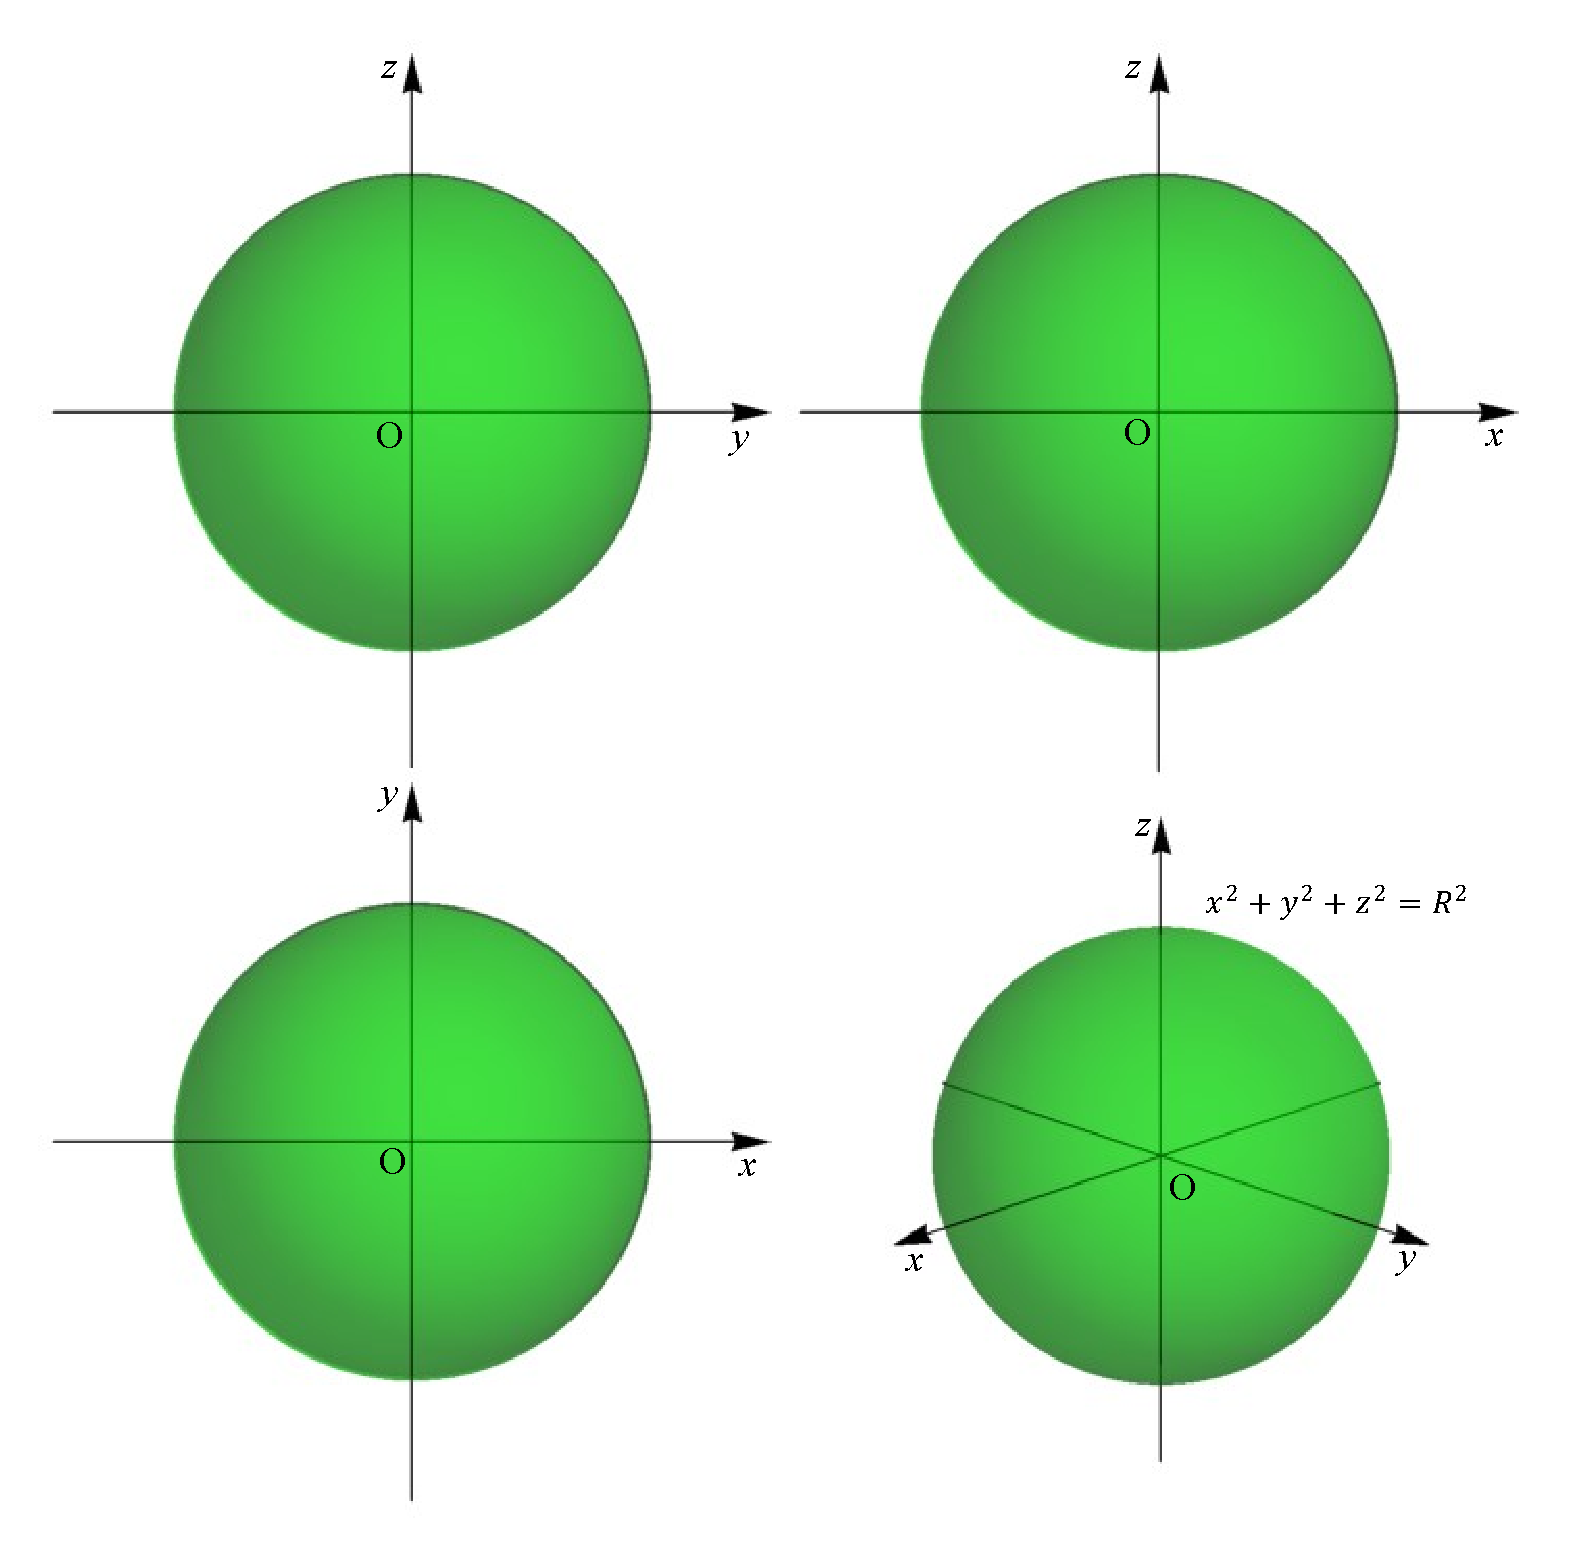
\includegraphics[height=0.70\textheight]{Figures20/Fig12-6-4-3.pdf}
\end{center}
\caption{习题12.6 4.(3)题图示}
\label{12-6-4-3}
\end{figure}
\end{enumerate}
\end{document}